% \iffalse
%  Local Variables:
%  mode: doctex
%  TeX-master: t
%  End:
% \fi
%
% \iffalse meta-comment
%
% Copyright (C) 2014-2015 by Kerui Wang <wkr@wangkerui.com>
% 
% Copyright (C) 2005-2011 by Ruini Xue <xueruini@gmail.com>
%
% This file may be distributed and/or modified under the
% conditions of the LaTeX Project Public License, either version 1.3a
% of this license or (at your option) any later version.
% The latest version of this license is in:
%
% http://www.latex-project.org/lppl.txt
%
% and version 1.3a or later is part of all distributions of LaTeX
% version 2004/10/01 or later.
%
% $Id$
%
% \fi
%
% \CheckSum{2012}
% \CharacterTable
%  {Upper-case    \A\B\C\D\E\F\G\H\I\J\K\L\M\N\O\P\Q\R\S\T\U\V\W\X\Y\Z
%   Lower-case    \a\b\c\d\e\f\g\h\i\j\k\l\m\n\o\p\q\r\s\t\u\v\w\x\y\z
%   Digits        \0\1\2\3\4\5\6\7\8\9
%   Exclamation   \!     Double quote  \"     Hash (number) \#
%   Dollar        \$     Percent       \%     Ampersand     \&
%   Acute accent  \'     Left paren    \(     Right paren   \)
%   Asterisk      \*     Plus          \+     Comma         \,
%   Minus         \-     Point         \.     Solidus       \/
%   Colon         \:     Semicolon     \;     Less than     \<
%   Equals        \=     Greater than  \>     Question mark \?
%   Commercial at \@     Left bracket  \[     Backslash     \\
%   Right bracket \]     Circumflex    \^     Underscore    \_
%   Grave accent  \`     Left brace    \{     Vertical bar  \|
%   Right brace   \}     Tilde         \~}
%
% \iffalse
%<*driver>
\ProvidesFile{sduthesis.dtx}[2014/05/05 0.1.0 Shandong University Thesis Template]
\documentclass[10pt]{ltxdoc}
\usepackage{dtx-style}
\EnableCrossrefs
\CodelineIndex
\RecordChanges
%\OnlyDescription
\begin{document}
\begin{CJK*}{UTF8}{song}
  \DocInput{\jobname.dtx}
\end{CJK*}
\end{document}
%</driver>
% \fi
%
% \GetFileInfo{\jobname.dtx}
% \MakeShortVerb{\|}
%
% \def\sduthesis{\textsc{Sdu}\-\textsc{Thesis}}
% \def\thuthesis{\textsc{Thu}\-\textsc{Thesis}}
% \def\TheHeaven{山东大学计算机学院信息安全所}
% \def\TheSatan{王克瑞}
% \def\pkg#1{\texttt{#1}}
%
% \DoNotIndex{\begin,\end,\begingroup,\endgroup}
% \DoNotIndex{\ifx,\ifdim,\ifnum,\ifcase,\else,\or,\fi}
% \DoNotIndex{\let,\def,\xdef,\newcommand,\renewcommand}
% \DoNotIndex{\expandafter,\csname,\endcsname,\relax,\protect}
% \DoNotIndex{\Huge,\huge,\LARGE,\Large,\large,\normalsize}
% \DoNotIndex{\small,\footnotesize,\scriptsize,\tiny}
% \DoNotIndex{\normalfont,\bfseries,\slshape,\interlinepenalty}
% \DoNotIndex{\hfil,\par,\hskip,\vskip,\vspace,\quad}
% \DoNotIndex{\centering,\raggedright}
% \DoNotIndex{\c@secnumdepth,\@startsection,\@setfontsize}
% \DoNotIndex{\ ,\@plus,\@minus,\p@,\z@,\@m,\@M,\@ne,\m@ne}
% \DoNotIndex{\@@par,\DeclareOperation,\RequirePackage,\LoadClass}
% \DoNotIndex{\AtBeginDocument,\AtEndDocument}
%
% \IndexPrologue{\section*{索引}%
%    \addcontentsline{toc}{section}{索~~~~引}}
%
% \renewcommand{\abstractname}{摘~~要}
% \renewcommand{\contentsname}{目~~录}
%
%
% \title{\sduthesis:山东大学学位论文模板\thanks{Shandong University \LaTeX{} Thesis Template.}}
% \author{{\fs \TheSatan}\\[5pt]{\fs \TheHeaven}\\[5pt] \texttt{wkr@wangkerui.com}}
% \date{v\fileversion\ (\filedate)}
% \maketitle\thispagestyle{empty}
%
%
% \begin{abstract}\noindent
%   本模板旨在建立一个简单易用的山东大学学位论文模板,全面支持硕士论文,有点支持博士论文,不支持本科论文。
% \end{abstract}
%
% \vskip2cm
% \def\abstractname{一些废话}
% \begin{abstract}
% \noindent
% \begin{enumerate}
% \item 本项目的发布遵守 DO WHAT THE FUCK YOU WANT TO PUBLIC LICENSE,使用前请认真阅读协议内容。
% \item 若项目内的文件有单独的LICENSE声明,则优先遵守该LICENSE。
% \item \sduthesis{} 脱胎于清华大学薛瑞尼老师的 \thuthesis{} 。可以说,没有 \thuthesis{} 就没有 \sduthesis{} ,在此表示由衷的感谢。
% \item 本模板与山东大学、山东大学教务处、山东大学研究生院均无关,为``民间''产品,所以此模板仅为参考实现,不保证格式审查老师
%   不提意见。任何由于使用本模板而引起的论文格式审查问题,本模板作者将尽量但不承诺提供帮助。
% \item 严禁用于商业目的(好像也没什么商业价值)。本条优先级高于第1、2条。
% \end{enumerate}
% \end{abstract}
%
%
% \clearpage
% \begin{multicols}{2}[
%   \section*{\contentsname}
%   \setlength{\columnseprule}{.4pt}
%   \setlength{\columnsep}{18pt}]
%   \tableofcontents
% \end{multicols}
%
% \clearpage
% \pagenumbering{arabic}
% \pagestyle{headings}
% \section{模板介绍}
% \sduthesis\ (\textbf{S}han\textbf{D}ong \textbf{U}niversity \textbf{Thesis}) 是为了帮助山东大学毕业
% 生撰写毕业论文而编写的 \LaTeX{} 论文模板。
% 如果你是硕士生,本模板正是你想要的;
% 如果你是博士生,本模板可能是你想要的(未做格式比对);
% 如果你是本科生,抱歉,本模板不是你的菜,不过你可能想看看
% \href{https://github.com/ChenMeng0518/sduthesis}{https://github.com/ChenMeng0518/sduthesis}。
%
% 本文档将尽量完整的介绍模板的使用方法,如有不清楚之处可以参考示例文档,欢迎感兴趣的同学出力完善此使用手册。由于个人水平有限,虽然现
% 在的这个版本基本上满足了学校的要求,但难免还存在不足之处,欢迎大家积极反馈。更希望师弟师妹们能够接手维护下去。
%
% {\color{blue}\fs 模板的作用在于减轻论文写作过程中格式调整的时间,其前提就是遵
%   守模板的用法,否则即使使用了 \sduthesis{} 也难以保证输出的论文符合学校规范。}
%
%
% \section{安装}
% \label{sec:installation}
%
% \subsection{下载}
% \sduthesis{} 相关链接:
% \begin{itemize}
% \item 主页:
% \href{https://github.com/wangkerui/sduthesis}{GitHub}
% \item 下载:
% \href{https://github.com/wangkerui/sduthesis/archive/master.zip}{.zip}
% \end{itemize}
%
% \sduthesis{} 的开发版本同样可以在 GitHub 上获得:
% \begin{shell}
% $ git clone git://github.com/wangkerui/sduthesis.git
% \end{shell}
%
% \subsection{模板的组成部分}
% 下表列出了 \sduthesis{} 的主要文件及其功能介绍:
%
% \begin{center}
%   \begin{longtable}{l|p{10cm}}
% \hline
% {\hei 文件(夹)} & {\hei 功能描述}\\\hline\hline
% \endfirsthead
% \hline
% {\hei 文件(夹)} & {\hei 功能描述}\\\hline\hline
% \endhead
% \endfoot
% \endlastfoot
% sduthesis.ins & 模板驱动文件 \\
% sduthesis.dtx & 模板文档代码的混合文件\\
% sduthesis.cls & 模板类文件(可由sduthesis.ins和sduthesis.dtx生成)\\
% sduthesis.cfg & 模板配置文件(可由sduthesis.ins和sduthesis.dtx生成)\\
% sdubib.bst & 参考文献样式文件\\\hline
% main.tex & 示例文档主文件\\
% ref/ & 示例文档参考文献目录\\
% data/ & 示例文档章节具体内容\\
% fig/ & 示例文档图片路径\\
% sdutils.sty & 为示例文档加载其它宏包\\\hline
% Makefile & self-explanation \\\hline
% Readme & self-explanation\\
% \textbf{sduthesis.pdf} & 用户手册(本文档)\\\hline
%   \end{longtable}
% \end{center}
%
% 需要说明几点:
% \begin{itemize}
% \item \emph{sduthesis.cls} 和 \emph{sduthesis.cfg} 可以
%   由 \emph{sduthesis.ins} 和 \emph{sduthesis.dtx} 生成,但为了降低新
%   手用户的使用难度,故将 cls和 cfg 一起发布。
% \item 使用前认真阅读文档:\emph{sduthesis.pdf}.
% \end{itemize}
% 
% \subsection{准备工作}
% \label{sec:prepare}
% 本模板用到以下宏包:
%
% \begin{center}
% \begin{minipage}{1.0\linewidth}\centering
% \begin{tabular}{*{6}{l}}\hline
%   ifxetex & xunicode & xltxtra & CJK\footnote{版本要求:$\geq$ v4.8.1} & xeCJK & \pkg{CJKpunct} \\
%   array & booktabs & longtable  &  amsmath & amssymb & ntheorem \\
%   indentfirst & paralist & txfonts & natbib & hyperref & hypernat \\
%   graphicx & \pkg{subfig}\footnote{版本要求:$\geq$2005/06/28 ver: 1.3} &
%   \pkg{caption}\footnote{版本要求:$\geq$2006/03/21 v3.0j} &
%   \pkg{sdubib.bst} & &\\\hline
% \end{tabular}
% \end{minipage}
% \end{center}
%
% 这些包在常见的 \TeX{} 系统中都有,如果没有请到 \url{www.ctan.org} 下载。推
% 荐 \TeX live。
%
%
% \subsection{开始安装}
% \label{sec:install}
%
% \subsubsection{生成模板}
% \label{sec:generate-cls}
% {\hei 说明:默认的发行包中已经包含了所有文件,可以直接使用。如果对如何由 dtx 生
%   成模板文件以及模板文档不感兴趣,请跳过本小节。}
%
% 模板解压缩后生成文件夹 sduthesis-VERSION\footnote{VERSION 为版本号。},其中包括:
% 模板源文件(sduthesis.ins 和 sduthesis.dtx),参考文献样式 sdubib.bst,示例文档
% (main.tex,sdutils.sty\footnote{可能用到但不一定用到的包以及一
%   些命令定义都放在这里面,以免 sduthesis.cls 过分臃
%   肿。},data/ 和 fig/ 和 ref/)。在使用之前需要先生成模板文件和配置文件
% (具体命令细节请参考 |Readme| 和 |Makefile|):
%
% \begin{shell}
% $ cd sduthesis-VERSION
% # 生成 sduthesis.cls 和 sduthesis.cfg
% $ latex sduthesis.ins
%
% # 下面的命令用来生成用户手册(本文档),一般不用执行
% $ latex sduthesis.dtx
% $ makeindex -s gind.ist -o sduthesis.ind sduthesis.idx
% $ makeindex -s gglo.ist -o sduthesis.gls sduthesis.glo
% $ latex sduthesis.dtx
% $ latex sduthesis.dtx  % 生成说明文档 sduthesis.dvi
% \end{shell}
%
%
% \subsubsection{dvi$\rightarrow$ps$\rightarrow$pdf}
% \label{sec:dvipspdf}
% 很多用户对 \LaTeX{} 命令执行的次数不太清楚,一个基本的原则是多次运行 \LaTeX{}
% 命令直至不再出现警告。下面给出生成示例文档的详细过程(\# 开头的行为注释),首先
% 来看经典的 \texttt{dvi$\rightarrow$ps$\rightarrow$pdf} 方式:
% \begin{shell}
% # 1. 发现里面的引用关系,文件后缀 .tex 可以省略
% $ latex main
%
% # 2. 编译参考文件源文件,生成 bbl 文件
% $ bibtex main
%
% # 3. 下面解决引用
% $ latex main
% # 如果是 GBK 编码,此处运行:
% # $ gbk2uni main  # 防止书签乱码
% $ latex main   # 此时生成完整的 dvi 文件
%
% # 4. 生成 ps
% $ dvips main.dvi
%
% # 5. 生成 pdf
% $ ps2pdf main.ps
% \end{shell}
%
% 模板已经把纸型信息写入目标文件,这样执行 \texttt{dvips} 时就可以避免由于遗忘
%  \texttt{-ta4} 参数而导致输出不合格的文件(因为 \texttt{dvips} 默认使用
%  letter 纸型)。
%
% \subsubsection{dvipdfm(x)}
% \label{sec:dvipdfmx}
% 如果使用 dvipdfm(x),那么在生成完整的 dvi 文件之后(参见上面的例子),可以直接得到 pdf:
% \begin{shell}%
% $ dvipdfm  main.dvi
% # 或者
% $ dvipdfmx  main.dvi
% \end{shell}
%
% \subsubsection{pdflatex}
% \label{sec:pdflatex}
% 如果使用 PDF\LaTeX,按照第~\ref{sec:dvipspdf} 节的顺序执行到第 3 步即可(将latex替换为pdflatex),不再经
% 过中间转换。
%
% 需要注意的是 PDF\LaTeX\ 不能处理常见的 EPS 图形,需要先用 epstopdf 将其转化
% 成 PDF。不过 PDF\LaTeX\ 增加了对 png,jpg 等标量图形的支持,比较方便。
%
% \subsubsection{xelatex}
% \label{sec:xelatex}
% XeTeX 最大的优势就是不再需要繁琐的字体配置。\sduthesis{} 通过 \pkg{xeCJK} 来控
% 制中文字体和标点压缩。模板里默认用的是 Windows 7 的六款字体(宋,黑,楷,仿宋,隶书,幼圆),
% 用户可以根据自己的实际情况方便的替换。
%
% Xe\LaTeX\ 的使用步骤同 PDF\LaTeX。
%
%
% \subsubsection{自动化过程}
% \label{sec:automation}
% 上面的例子只是给出一般情况下的使用方法,可以发现虽然命令很简单,但是每次都输入
% 的话还是非常罗嗦的,所以 \sduthesis{} 还提供了一些自动处理的文件。
%
% 我们提供了一个简单的 \texttt{Makefile}:
% \begin{shell}
% $ make clean
% $ make ins       # 生成 sduthesis.cls 和 sduthesis.cfg
% $ make doc       # 生成说明文档 sduthesis.pdf(本文档)
% $ make thesis    # 生成示例文档 main.pdf
% \end{shell}
%
% 如果使用 Windows 平台,推荐安装Cygwin或者MinGW后再使用make命令。
%
% \texttt{Makefile} 默认采用 \LaTeX\ 编译,可以根据自己的需要指定编译参数,如:
% \begin{shell}
% $ make thesis METHOD=pdftex  # 采用pdfLaTeX 编译
% \end{shell}
%
%
% \subsection{升级}
% \label{sec:updgrade}
% \sduthesis{} 升级非常简单,下载最新的版本,
% 将 sduthesis.ins,sduthesis.dtx 和sdubib.bst 拷贝至工作目录覆盖相应的文件,然后
% 运行:
% \begin{shell}
% $ latex sduthesis.ins
% \end{shell}
%
% 生成新的类文件和配置文件即可。当然也可以直接拷贝 sduthesis.cls, sduthesis.cfg
% 和 sdubib.bst,免去上面命令的执行。只要明白它的工作原理,这个不难操作。
%
%
% \section{使用说明}
% \label{sec:usage}
% 本手册假定用户已经能处理一般的 \LaTeX{} 文档,并对 \BibTeX{} 有一定了解。如果你
% 从来没有接触过 \TeX 和 \LaTeX,建议先学习相关的基础知识。磨刀不误砍柴工!
%
% \subsection{关于提问}
% \label{sec:howtoask}
% \begin{itemize}\addtolength{\itemsep}{-5pt}
% \item 请先阅读\ref{sec:qanda}节
% \item 请使用\href{https://github.com/wangkerui/dartscorer/issues}{Github Issues}
% \end{itemize}
%
% \subsection{\sduthesis{} 示例文件}
% \label{sec:userguide1}
% 模板核心文件只有三个:sduthesis.cls,sduthesis.cfg 和 sdubib.bst,但是如果没有
% 示例文档用户会发现很难下手。所以推荐新用户从模板自带的示例文档入手,里面包括了
% 论文写作用到的所有命令及其使用方法,只需要用自己的内容进行相应替换就可以。对于
% 不清楚的命令可以查阅本手册。下面的例子描述了模板中章节的组织形式,来自于示例文
% 档,具体内容可以参考模板附带的 main.tex 和 data/。
%
% \begin{example}
% \documentclass[master]{sduthesis}
% % \documentclass[%
% %   master|doctor,              % mandatory option
% %   xetex|pdftex|dvips|dvipdfm, % optional
% %   secret,                     % optional
% %   equival,engineer            % optional
% %   openany|openright,          % optional
% %   arial,arialtoc,arialtitle   % optional
% % ]{sduthesis}
% 
% % 用到的宏包都统一放到了sdutils中,
% % 可以根据自己的实际在sdutils.sty中添加或者删除。
% \usepackage{sdutils}
% 
% \begin{document}
% % 图片目录
% \graphicspath{{fig/}}
% 
% 
% %%% 1.前序部分
% \frontmatter
% % 封面,博士有英文封面
% %%% Local Variables:
%%% mode: latex
%%% TeX-master: "../main.tex"
%%% End:

\catalognumber{TP393}
\schoolnumber{10422}
\secretlevel{内部} \secretyear{5}% 必须打开secret选项才有效
\studentnumber{201113XXX}

\ctitle{\sduthesis 示例文档}
\etitle{AN EXAMPLE DOCUMENT OF \sduthesis}
\cauthor{王克瑞}
\cdepartment{计算机科学与技术学院}
\cmajor{计算机应用技术}
\csupervisor{某某某\hspace{1em}教授}
\ccosupervisor{某某\hspace{1em}副教授}
% 日期自动生成,如果你要自己写就改这个cdate
\cdate{\the\year 年\the\month 月\the\day 日}

% 以下是博士的英文封面项。如果你是硕士,never mind
\eauthor{Wang Kerui}
\esupervisor{Prof.\:\ Mou Moumou}
\ecosupervisor{Prof.\:\ Mou Mou}
\eaddress{Shandong University, Jinan, Shandong, P.R.China}
\edate{April 30, 2014}

% \makecover
% 
% % 原创性声明和关于学位论文使用授权的声明
% %%%
%%% Originality Statement & Authorization Statement.
%%%
%%% File:   data/statement.tex
%%% Date:   4/23/2014
%%% Author: wkr@wangkerui.com
%%%

\originalitytitle{原\quad 创\quad 性\quad 声\quad 明}
\originalitycontent{本人郑重声明:所呈交的学位论文,是本人在导师的指导下,独立进行研究所取得的成果。除文中已经注明引用的内容外,本论文不包含任何其他个人或集体已经发表或撰写过的科研成果。对本文的研究作出重要贡献的个人和集体,均已在文中以明确方式标明。本声明的法律责任由本人承担。}

\authorizationtitle{关于学位论文使用授权的声明}
\authorizationcontent{本人同意学校保留或向国家有关部门或机构送交论文的印刷件和电子版,允许论文被查阅和借阅;本人授权山东大学可以将本学位论文的全部或部分内容编入有关数据库进行检索,可以采用影印、缩印或其他复制手段保存论文和汇编本学位论文。}
\authorizationaddon{(保密论文在解密后应遵守此规定)}

%%%
%%% End of file.
%%%

% \makestatement
% 
% % 目录
% \begin{contents}
% \tableofcontents%  中文目录
% \tableofecontents% 英文目录
% \end{contents}
% 
% % 摘要(包括中文摘要和英文摘要)
% %%%
%%% File:       abstract.tex
%%% TeX-Master: ../main.tex
%%% Desc:       Including Chinese & English Abstract.
%%%

% 中文摘要
\chapter{摘\hspace{1em}要}
\echapter{Chinese Abstract}
这里写摘要。请注意:务必先浏览 sduthesis.pdf 的前 4 章,然后再结合本示例文档写作论文。

本示例文档主要示例如何使用本模板排版,基本上和标准类模板没差。包括,章节标题,英文目录,公式、算法,插图、表格,定义、定理和证明环境等。

填充废话。

豫章故郡,洪都新府。星分翼轸(zhěn),地接衡庐。襟三江而带五湖,控蛮荆而引瓯(ōu)越。物华天宝,龙光射牛斗之墟;人杰地灵,徐孺下陈蕃(fān)之榻(tà)。雄州雾列,俊采星驰。台隍(huáng)枕夷夏之交,宾主尽东南之美。都督阎公之雅望,棨(qǐ)戟(jǐ)遥临;宇文新州之懿(yì)范,襜(chān)帷(wéi)暂驻。十旬休暇,胜友如云;千里逢迎,高朋满座。腾蛟起凤,孟学士之词宗;紫电青霜,王将军之武库。家君作宰,路出名区;童子何知,躬逢胜饯。

时维九月,序属三秋。潦(lǎo)水尽而寒潭清,烟光凝而暮山紫。俨(yǎn)骖(cān)騑(fēi)于上路,访风景于崇阿(ē)。临帝子之长洲,得天人之旧馆。层峦耸翠,上出重霄;飞阁流丹,下临无地。鹤汀(tīng)凫(fú)渚(zhǔ),穷岛屿之萦回;桂殿兰宫,即冈峦之体势。

披绣闼(tà),俯雕甍(méng),山原旷其盈视,川泽纡其骇瞩。闾阎(lǘ yán)扑地,钟鸣鼎食之家;舸(gě)舰弥津,青雀黄龙之轴(通:舳zhú)。云销雨霁,彩彻区明。落霞与孤鹜齐飞,秋水共长天一色。渔舟唱晚,响穷彭蠡(lǐ)之滨,雁阵惊寒,声断衡阳之浦。

遥襟甫畅,逸兴遄(chuán)飞。爽籁发而清风生,纤歌凝而白云遏(è)。睢(suī)园绿竹,气凌彭泽之樽(zūn);邺(yè)水朱华,光照临川之笔。四美具,二难并。穷睇眄(dìmiǎn)于中天,极娱游于暇日。天高地迥(jiǒng),觉宇宙之无穷;兴尽悲来,识盈虚之有数。望长安于日下,目吴会(kuài)于云间。地势极而南溟(míng)深,天柱高而北辰远。关山难越,谁悲失路之人;萍水相逢,尽是他乡之客。怀帝阍(hūn)而不见,奉宣室以何年?

嗟乎!时运不齐,命途多舛(chuǎn)。冯唐易老,李广难封。屈贾谊于长沙,非无圣主;窜梁鸿于海曲,岂乏明时?所赖君子见机,达人知命。老当益壮,宁移白首之心?穷且益坚,不坠青云之志。酌贪泉而觉爽,处涸辙(hézhé)以犹欢。北海虽赊(shē),扶摇可接;东隅(yú)已逝,桑榆非晚。孟尝高洁,空余报国之情;阮籍猖狂,岂效穷途之哭!

勃,三尺微命,一介书生。无路请缨,等终军之弱冠;有怀投笔,慕宗悫(què)之长风。舍簪(zān)笏(hù)于百龄,奉晨昏于万里。非谢家之宝树,接孟氏之芳邻。他日趋(qū)庭,叨(tāo)陪鲤对;今兹捧袂,喜托龙门。杨意不逢,抚凌云而自惜;钟期既遇,奏流水以何惭?

呜乎!胜地不常,盛筵难再;兰亭已矣,梓(zǐ)泽丘墟。临别赠言,幸承恩于伟饯;登高作赋,是所望于群公。敢竭鄙怀,恭疏短引;一言均赋,四韵俱成。请洒潘江,各倾陆海云尔:

\begin{center}
滕王高阁临江渚,佩玉鸣鸾罢歌舞。

画栋朝飞南浦云,珠帘暮卷西山雨。

闲云潭影日悠悠,物换星移几度秋。

阁中帝子今何在?槛外长江空自流。
\end{center}

废话填充完毕。你可以用\verb|\vspace{2em}|或者\verb|\vskip 2em|来控制和关键字的距离;还可以在前面加上\verb|\noindent|来取消关键字行的缩进。

% 中文关键字
\vspace{2em}
\noindent\textbf{关键字}:滕王阁序;王勃;赋


% English Abstract
\chapter{ABSTRACT}
\echapter{ABSTRACT}
Here is English abstract. (We fill out with a bunch of crap.)

Ever since the "Heartbleed" flaw in encryption protocol OpenSSL was made public on April 7 in the US there have been various questions about who knew what and when.

Fairfax Media has spoken to various people and groups involved and has compiled the below timeline.

If you have further information or corrections - especially information about what occurred prior to March 21 at Google - please email the author: bgrubb@fairfaxmedia.com.au. Click here for his PGP key.

All times are in US Pacific Daylight Time

Advertisement
Friday, March 21 or before - Neel Mehta of Google Security discovers Heartbleed vulnerability.

Friday, March 21 10.23 -  Bodo Moeller and Adam Langley of Google commit a patch for the flaw (This is according to the timestamp on the patch file Google created and later sent to OpenSSL, which OpenSSL forwarded to Red Hat and others). The patch is then progressively applied to Google services/servers across the globe.

Monday, March 31 or before - Someone tells content distribution network CloudFlare about Heartbleed and they patch against it. CloudFlare later boasts on its blog about how they were able to protect their clients before many others. CloudFlare chief executive officer Matthew Prince would not tell Fairfax how his company found out about the flaw early. "I think the most accurate reporting of events with regard to the disclosure process, to the extent I know them, was written by Danny over at the [Wall Street Journal]," he says. The article says CloudFlare was notified of the bug the week before last and made the recommended fix "after signing a non-disclosure agreement". In a seperate article, The Verge reports that a CloudFlare staff member "got an alarming message from a friend" which requested that they send the friend their PGP email encryption key as soon as possible. "Only once a secure channel was established and a non-disclosure agreement was in place could he share the alarming news" about the bug, The Verge reported. On April 17, CloudFlare says in a blog that when it was informed it did not know then that it was among the few to whom the bug was disclosed before the public announcement. "In fact, we did not even know the bug's name. At that time we had simply removed TLS heartbeat functionality completely from OpenSSL..."

Tuesday, April 1 - Google Security notifies "OpenSSL team members" about the flaw it has found in OpenSSL, which later becomes known as "Heartbleed", Mark Cox at OpenSSL says on social network Google Plus.

Tuesday, April 1 04:09 - "OpenSSL team members" forward Google's email to OpenSSL's "core team members". Cox at OpenSSL says the following on Google Plus: "Original plan was to push [a fix] that week, but it was postponed until April 9 to give time for proper processes." Google tells OpenSSL, according to Cox, that they had "notified some infrastructure providers under embargo". Cox says OpenSSL does not have the names of providers Google told or the dates they were told. Google declined to tell Fairfax which partners it had told. "We aren't commenting on when or who was given a heads up," a Google spokesman said.

Wednesday, April 2 ~23:30  - Finnish IT security testing firm Codenomicon separately discovers the same bug that Neel Mehta of Google found in OpenSSL. A source inside the company gives Fairfax the time it was found as 09:30 EEST April 3, which converts to 23:30 PDT, April 2.

Thursday, April 3 04:30 - Codenomicon notifies the National Cyber Security Centre Finland (NCSC-FI) about its discovery of the OpenSSL bug. Codenomicon tells Fairfax in a statement that they're not willing to say whether they disclosed the bug to others. "We have strict [non-disclosure agreements] which do not allow us to discuss any customer engagements. Therefore, we do not want to weigh in on the disclosure debate," a company spokeswoman says. A source inside the company later tells Fairfax: "Our customers were not notified. They first learned about it after OpenSSL went public with the information."

Friday, April 4 - Content distribution network Akamai patches its servers. They initially say OpenSSL told them about bug but the OpenSSL core team denies this in an email interview with Fairfax. Akamai updates its blog after the denial - prompted by Fairfax - and Akamai's blog now says an individual in the OpenSSL community told them. Akamai's chief security officer, Andy Ellis, tells Fairfax: "We've amended the blog to specific [sic] a member of the community; but we aren't going to disclose our source."  It's well known a number of OpenSSL community members work for companies in the tech sector that could be connected to Akamai.

Friday, April 4 - Rumours begin to swirl in open source community about a bug existing in OpenSSL, according to one security person at a Linux distribution Fairfax spoke to. No details were apparent so it was ignored by most.

Saturday, April 5 15:13 - Codenomicon purchases the Heartbleed.com domain name, where it later publishes information about the security flaw.

Saturday, April 5 16:51 - OpenSSL (not public at this point) publishes this (since taken offline) to its Git repository.

Sunday, April 6 02:30 - The National Cyber Security Centre Finland asks the CERT Coordination Centre (CERT/CC) in America to be allocated a common vulnerabilites exposure (CVE) number "on a critical OpenSSL issue" without disclosing what exactly the bug is. CERT/CC is located at the Software Engineering Institute, a US government funded research centre operated by Carnegie Mellon University. The centre was created in in 1988 at DARPA's direction in response to the Morris worm incident.

Sunday,  April 6 ~22:56 - Mark Cox of OpenSSL (who also works for Red Hat and was on holiday) notifies Linux distribution Red Hat about the Heartbleed bug and authorises them to share details of the vulnerability on behalf of OpenSSL to other Linux operating system distributions.

Sunday, April 6 22.56 - Huzaifa Sidhpurwala (who works for Red Hat) adds a (then private) bug to Red Hat's bugzilla.

Sunday, April 6 23.10 - Huzaifa Sidhpurwala sends an email about the bug to a private Linux distribution mailing list with no details about Heartbleed but an offer to request them privately under embargo. Sidhpurwala says in the email that the issue would be made public on April 9. Cox of OpenSSL says on Google Plus: "No details of the issue are given: just affected versions [of OpenSSL]. Vendors are told to contact Red Hat for the full advisory under embargo."

Sunday, April 6 ~23:10 - A number of people on the private mailing list ask Sidhpurwala, who lives in India, for details about the bug. Sidhpurwala gives details of the issue, advisory, and patch to the operating system vendors that replied under embargo. Those who got a response included SuSE (Monday, April 7 at 01:15), Debian (01:16), FreeBSD (01:49) and AltLinux (03:00). “Some other [operating system] vendors replied but [Red Hat] did not give details in time before the issue was public," Cox said. Sidhpurwala was asleep during the time the other operating system vendors requested details. "Some of them mailed during my night time. I saw these emails the next day, and it was pointless to answer them at that time, since the issue was already public," Sidhpurwala says. Those who attempted to ask and were left without a response included Ubuntu (asked at 04:30), Gentoo (07:14) and Chromium (09:15), says Cox. 

Prior to Monday, April 7 or early April 7 - Facebook gets a heads up, people familiar with matter tell the Wall Street Journal. Facebook say after the disclosure: "We added protections for Facebook’s implementation of OpenSSL before this issue was publicly disclosed, and we're continuing to monitor the situation closely." An article on The Verge suggests Facebook got an encrypted email message from a friend in the same way CloudFlare did.

Monday, April 7 08.19 - The National Cyber Security Centre Finland reports Codenomicon's OpenSSL "Heartbleed" bug to OpenSSL core team members Ben Laurie (who works for Google) and Mark Cox (Red Hat) via encrypted email.

Monday, April 7 09.11 - The encrypted email is forwarded to the OpenSSL core team members, who then decide, according to Cox, that "the coincidence of the two finds of the same issue at the same time increases the risk while this issue remained unpatched. OpenSSL therefore released updated packages [later] that day."

Monday, April 7 09:53 - A fix for the OpenSSL Heartbleed bug is committed to OpenSSL's Git repository (at this point private). Confirmed by Red Hat employee: "At this point it was private."

Monday, April 7 10:21:29 - A new OpenSSL version is uploaded to OpenSSL's web server with the filename "openssl-1.0.1g.tgz".

Monday, April 7 10:27 - OpenSSL publishes a Heatbleed security advisory on its website (website metadata shows time as 10:27 PDT).

Monday, April 7 10:49 - OpenSSL issues a Heartbleed advisory via its mailing list. It takes time to get around.

Monday, April 7 11:00 - CloudFlare posts a blog entry about the bug.

Monday, April 7 12:23 - CloudFlare tweets about its blog post.

Monday, April 7 12:37 - Google's Neel Mehta comes out of Twitter hiding to tweet about the OpenSSL flaw.

Monday, April 7 13:13 - Codenomicon tweets they found bug too and link to their Heartbleed.com website.

Monday, April 7 ~13:13 - Most of the world finds out about the issue through heartbleed.com.

Monday, April 7 15:01 - Ubuntu comes out with patch.

Monday, April 7 23.45 - The National Cyber Security Centre Finland issues a security advisory on its website in Finnish.

Monday, April 8 ~00:45 - The National Cyber Security Centre Finland issues a security advisory on its website in English.

Tuesday, April 9 - A Red Hat technical administrator for cloud security, Kurt Seifried, says in a public mailing list that Red Hat and OpenSSL tried to coordinate disclosure. But Seifried says things "blew up" when Codenomicon reported the bug too. "My understanding is that OpenSSL made this public due to additional reports. I suspect it boiled down to 'Group A found this flaw, reported it, and has a reproducer, and now Group B found the same thing independently and also has a reproducer. Chances are the bad guys do as well so better to let everyone know the barn door is open now rather than wait 2 more days'. But there may be other factors I'm not aware [of],” Seifried says.

Wednesday, April 9 - A Debian developer, Yves-Alexis Perez, says on the same mailing list: "I think we would have managed to handle it properly if the embargo didn't break."

Wednesday, April 9 - Facebook and Microsoft donate \$ US15,000 to Neel Mehta via the Internet Bug Bounty program for finding the OpenSSL bug. Mehta gives the funds to the Freedom of the Press Foundation.

Monday, April 14 ~12.30pm - The Guardian reports a mothers forum with 1.5 million users called Mumsnets is impacted by Heartbleed. A "hacker" reportedly breached the admin's user account.

Monday, April 14 - the Canada Revenue Agency announces social insurance numbers of approximately 900 taxpayers were removed from its systems by someone exploiting the Heartbleed vulnerability.

Wednesday, April 16 - A Canadian teen is arrested for stealing tax data with Heartbleed.

Who knew of heatbleed prior to release? Google (March 21 or prior), CloudFlare (March 31 or prior), OpenSSL (April 1), Codenomicon (April 2), National Cyber Security Centre Finland (April 3), Akamai (April 4 or earlier) and Facebook (no date given).

Who knew hours before public release? SuSE, Debian, FreeBSD and AltLinux.

Who didn't know until public release? Many, including Amazon Web Services, Twitter, Yahoo, Ubuntu, Cisco, Juniper, Pinterest, Tumblr, GoDaddy, Flickr, Minecraft, Netflix, Soundcloud, Commonwealth Bank of Australia (main website, not net banking website), CERT Australia website, Instagram, Box, Dropbox, GitHub, IFTTT, OKCupid, Wikipedia, Wordpress and Wunderlist.


% English Keywords
\vspace{2em}
\noindent\textbf{Keywords}: heartbleed; OpenSSL; https; Google

%%%
%%% End of File
%%%

% 
% % 符号说明
% % 本章不会出现在目录中

\begin{denotation}[2.0cm]% 默认2.5cm
  \item[$E$] 能量
  \item[$m$] 质量
  \item[$c$] 光速
\end{denotation}

% 
% 
% %%% 2.正文部分
% \mainmatter
% %%% Local Variables:
%%% mode: latex
%%% TeX-master: ../main.tex
%%% End:

% \e<sectionlevel> (如 \echapter, \esection, \esubsection) 用于生成英文目录
\chapter{一级标题}
\echapter{English Chapter Name}
\label{cha:cha}
示例章节命令和参考文献的用法。注意:本文档仅是示例,请一定先阅读详细的说明文档 sduthesis.pdf 。


\section{二级标题}
\esection{English Section Name}
这是二级标题。

所有级别的标题都可以使用带 e 的版本生成英文目录(四级标题除外)。

\subsection{三级标题}
\esubsection{English Subsection Name}
这是三级标题。

\subsubsection{四级标题}
\esubsubsection{Si Ji Biao Ti}
四级标题不会出现在目录中。

另外,上述标题带 * 号的版本都不带编号,不计入目录。

\subsubsection*{starsubsubsection}
本节是带 * 号版本的例子。


\section{引用用法}
\esection{References}
参考文献有两种用法:一是上标模式,如这是上标模式\cite{cnproceed},二是正文模式,如文献\onlinecite{cnarticle}指出...。

\section{本文的结构}
\esection{Paper Structure}
本文第\ref{cha:cha}章示例章节命令和参考文献的用法。

本文第\ref{cha:example}章示例正文的用法,如插图和表格,公式和算法,定义、定理和证明环境等。

%%%
%%% End of File
%%%

% %%% Local Variables:
%%% mode: latex
%%% TeX-master: ../main.tex
%%% End:

\chapter{用法示例}
\echapter{Example}
\label{cha:example}

\section{插图}
\esection{Figure}

\begin{figure}[!htbp]
  \centering
  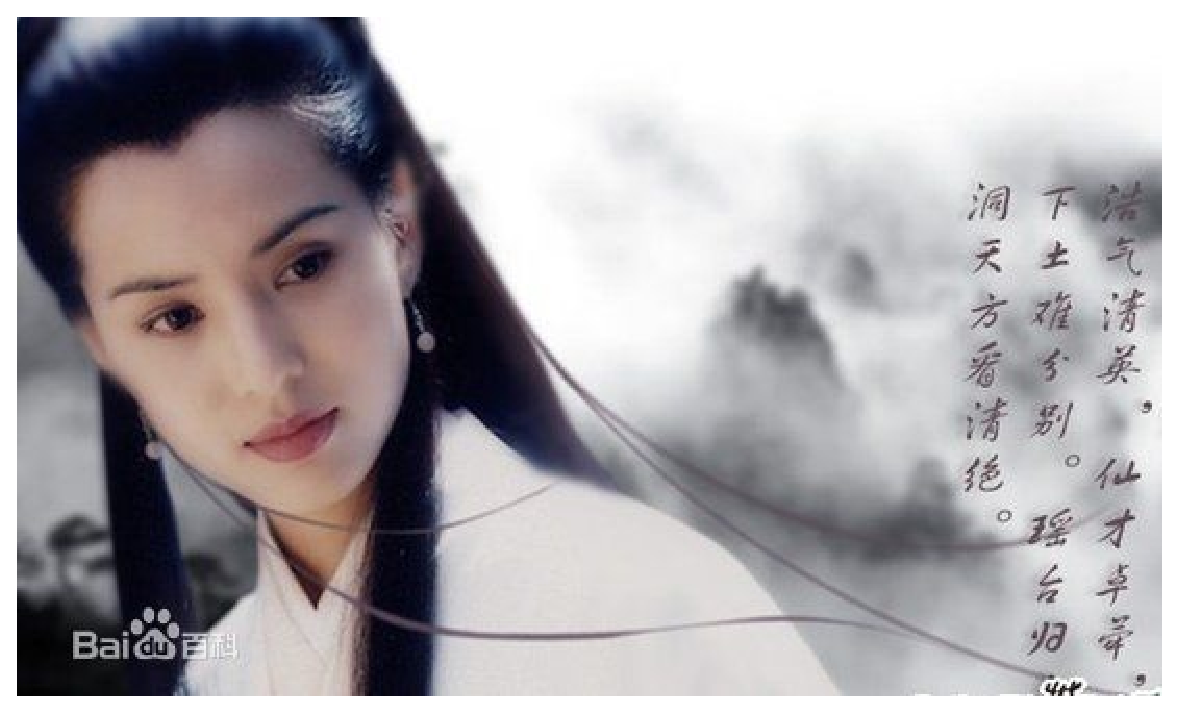
\includegraphics[width=\textwidth]{lrt}
  \caption{香中别有韵,清极不知寒}
  \label{fig:lrt}    
\end{figure}

图\ref{fig:lrt}是一个插图的例子。

图\ref{fig:lrt2}是另一个插图的例子。

\begin{figure}[!htbp]
  \centering
  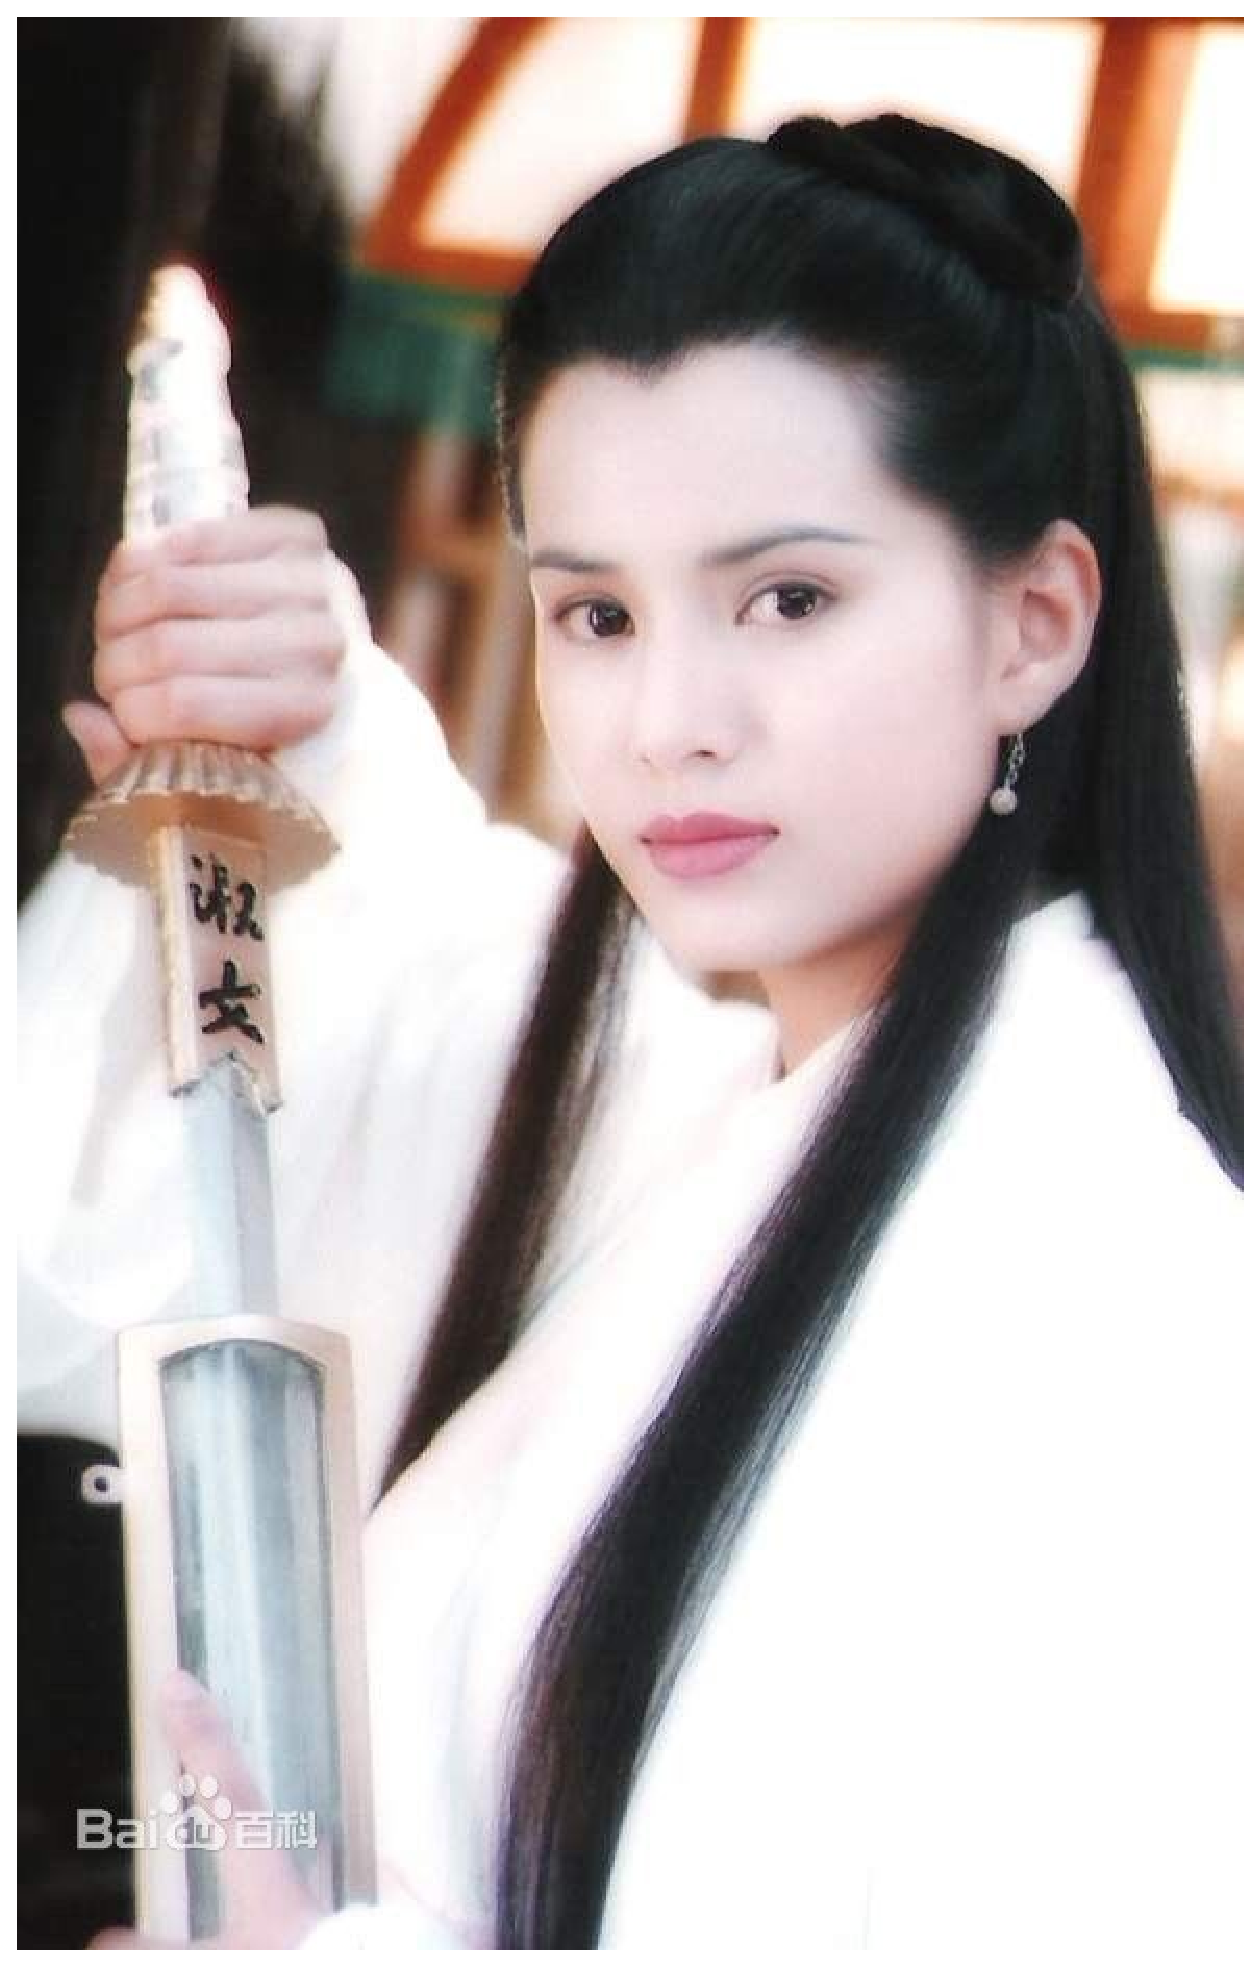
\includegraphics[height=3.5in]{lrt2}
  \caption{翩若游龙,宛若惊鸿}
  \label{fig:lrt2}    
\end{figure}


\section{表格}
\esection{Table}

\begin{table}[htbp]
  \centering
  \caption{这是一个自动编号的表格例子}
  \label{tab:tbl}
  \begin{tabular}[c]{|c|m{0.8in}|c|c|c|c|c|}\hline
    \multicolumn{2}{|c|}{Network Topology} & \# of nodes & 
    \multicolumn{3}{c|}{\# of clients} & Server \\\hline
    GT-ITM & Waxman Transit-Stub & 600 &
    \multirow{2}{2em}{2\%}& 
    \multirow{2}{2em}{10\%}& 
    \multirow{2}{2em}{50\%}& 
    \multirow{2}{1.2in}{Max. Connectivity}\\\cline{1-3}
    \multicolumn{2}{|c|}{Inet-2.1} & 6000 & & & &\\\hline
    \multirow{2}{1in}{blabla} & ban  & ban &\multicolumn{4}{c|}{\multirow{2}*{\sduthesis}}\\\cline{2-3}
    & \multicolumn{2}{c|}{ABCDEF} &\multicolumn{4}{c|}{} \\\hline
\end{tabular}  
\end{table}


\section{公式}
\esection{Equation}

首先,有行内公式,如$H~:~\mathcal{C}_n \rightarrow \mathcal{D}_n = \{0,1\}^\lambda$。

然后,有独立成行的不带编号的公式,如
$$
\forall\mathbf{y}\in\Lambda,\quad\mathcal{D}_{\Lambda,s,\mathbf{c}}(\mathbf{y})=\frac{\rho_{s,\mathbf{c}}(\mathbf{y})}{\rho_{s,\mathbf{c}}(\Lambda)}
$$

接下来,就是正常的带编号的公式了,如
\begin{equation}
  \mathbf{Adv}^{eu\mbox{-}acma}_{\Pi}(\mathcal{A}) =  \Pr \left[\mathsf{Sig}\mbox{-}forge_{\mathcal{A},\Pi}(n) = 1 \right] \leq \mathsf{negl}(n).
\end{equation}


\section{算法}
\esection{Algorithm}

\begin{algorithm}
  \caption{算法名称}
\label{alg:alg}
  \algorithmicrequire 输入参数 \\
  \algorithmicensure 输出结果
  \begin{enumerate}
    \item 步骤1
    \item 步骤2
    \item 步骤3
  \end{enumerate}
\end{algorithm}


\section{定义}
\esection{Definition}

\begin{definition}[格]
\label{def:lattice}
给定一组线性无关的向量$\mathbf{B}=\left\{\mathbf{b}_1,\cdots,\mathbf{b}_n\right\}\in\mathbb{R}^{m\times n}$,定义
\begin{equation}
\mathcal{L}(\mathbf{B})=\mathcal{L}(\mathbf{b}_1,\cdots,\mathbf{b}_n)=\left\{\sum_{i\in[n]}x_i\mathbf{b}_i\mid x_i\in\mathbb{Z}\right\}
\end{equation}
为$\mathbf{B}$上的格。其中,线性无关向量组$\mathbf{B}$称作格的\textit{基},$m$和$n$分别称作格的\textit{维}和\textit{秩}。
\end{definition}

定义\ref{def:lattice}是一个定义的例子。


\section{定理}
\esection{Theorem}

\begin{lemma}
\label{lem:basis}
      $\{\mathbf{b}_1,\cdots,\mathbf{b}_n\}$是(有序)基,另一有序基$\{\mathbf{d}_n,\cdots,\mathbf{d}_1\}$是前者对偶基的逆序,那么$\tilde{\mathbf{d}_i}=\tilde{\mathbf{b}_i}/\lVert\tilde{\mathbf{b}_i}\rVert^2(i\in[n])$。
\end{lemma}

引理\ref{lem:basis}是一个引理的例子。其它定理环境参见 sduthesis.pdf 3.6节数学环境。


\section{证明}
\esection{Proof}

\begin{proof}
这是一个证明环境,证明结束的地方会显示一个小黑块。
\end{proof}


\section{其它}
\esection{Others}

不带编号列表:

\begin{itemize}
  \item 无编号
  \item 每项前面有小圆点
  \item 可嵌套
  \begin{itemize}
    \item 最多嵌套3层
    \begin{itemize}
      \item 最多嵌套3层
      \begin{itemize}
        \item 最多嵌套3层
      \end{itemize}
    \end{itemize}
  \end{itemize}
  \item 无编号
\end{itemize}

编号列表:

\begin{enumerate}
  \item 有编号
  \item 可嵌套
  \begin{enumerate}
    \item 第1层嵌套
    \item 最多嵌套3层
    \begin{enumerate}
      \item 最多嵌套3层
        \begin{enumerate}
          \item 最多嵌套3层
        \end{enumerate}
    \end{enumerate}
  \end{enumerate}
  \item 这是顶层条目
\end{enumerate}


%%%
%%% End of File
%%%

% 
% 
% %%% 3.后续部分
% \backmatter
% % 附录
% \begin{appendix}
% %%% Local Variables: 
%%% mode: latex
%%% TeX-master: "../main"
%%% End: 

\chapter{特殊浮动对象}
\echapter{Special Float Object}
\label{cha:speobj}
如果附录中的公式不想让它出现在公式索引中,那就请用 \verb|\tag*{xxx}|

\begin{equation}\tag*{(123)} 
\left\{\begin{array}{l}
\max \,\,f(x)\\[0.1 cm]
\mbox{subject to:} \\ [0.1 cm]
\qquad g_j(x)\le 0,\quad j=1,2,\cdots,p
\end{array}\right.
\end{equation}

\begin{table}[ht]
  \centering
  \caption*{Table~111\hskip1em This is an example for manually numbered table, which
    would not appear in the list of tables}
  \label{tab:badtabular2}
  \begin{tabular}[c]{|c|m{0.8in}|c|c|c|c|c|}\hline
    \multicolumn{2}{|c|}{Network Topology} & \# of nodes & 
    \multicolumn{3}{c|}{\# of clients} & Server \\\hline
    GT-ITM & Waxman Transit-Stub & 600 &
    \multirow{2}{2em}{2\%}& 
    \multirow{2}{2em}{10\%}& 
    \multirow{2}{2em}{50\%}& 
    \multirow{2}{1.2in}{Max. Connectivity}\\\cline{1-3}
    \multicolumn{2}{|c|}{Inet-2.1} & 6000 & & & &\\\hline
    \multirow{2}{1in}{blahblah} & jin  & jin &\multicolumn{4}{c|}{\multirow{2}*{\sduthesis}}\\\cline{2-3}
    & \multicolumn{2}{c|}{ABCDEF} &\multicolumn{4}{c|}{} \\\hline
\end{tabular}  
\end{table}

\begin{figure}[h]
  \centering
  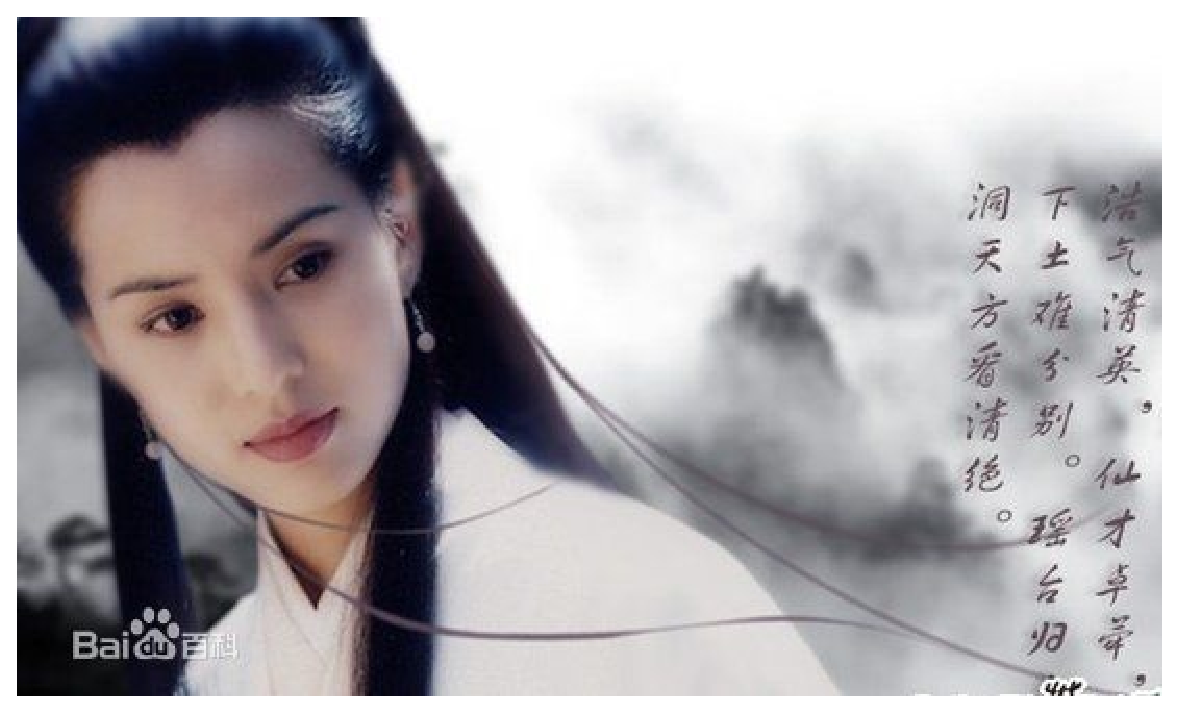
\includegraphics[width=\textwidth]{lrt}
  \caption*{Figure~123\hskip1em This is an example for manually numbered figure,
    which would not appear in the list of figures}
  \label{tab:badfigure2}    
\end{figure}

\begin{table}[ht]
\centering
  \centering
  \caption*{表~222\hskip1em 这是手动编号但不出现在索引中的表格例子}
  \label{tab:badtabular3}
  \begin{tabular}[c]{|c|m{0.8in}|c|c|c|c|c|}\hline
    \multicolumn{2}{|c|}{Network Topology} & \# of nodes & 
    \multicolumn{3}{c|}{\# of clients} & Server \\\hline
    GT-ITM & Waxman Transit-Stub & 600 &
    \multirow{2}{2em}{2\%}& 
    \multirow{2}{2em}{10\%}& 
    \multirow{2}{2em}{50\%}& 
    \multirow{2}{1.2in}{Max. Connectivity}\\\cline{1-3}
    \multicolumn{2}{|c|}{Inet-2.1} & 6000 & & & &\\\hline
    \multirow{2}{1in}{blah} & blah  & jin &\multicolumn{4}{c|}{\multirow{2}*{\sduthesis}}\\\cline{2-3}
    & \multicolumn{2}{c|}{ABCDEF} &\multicolumn{4}{c|}{} \\\hline
\end{tabular}  
\end{table}

\begin{figure}[!htbp]
  \centering
  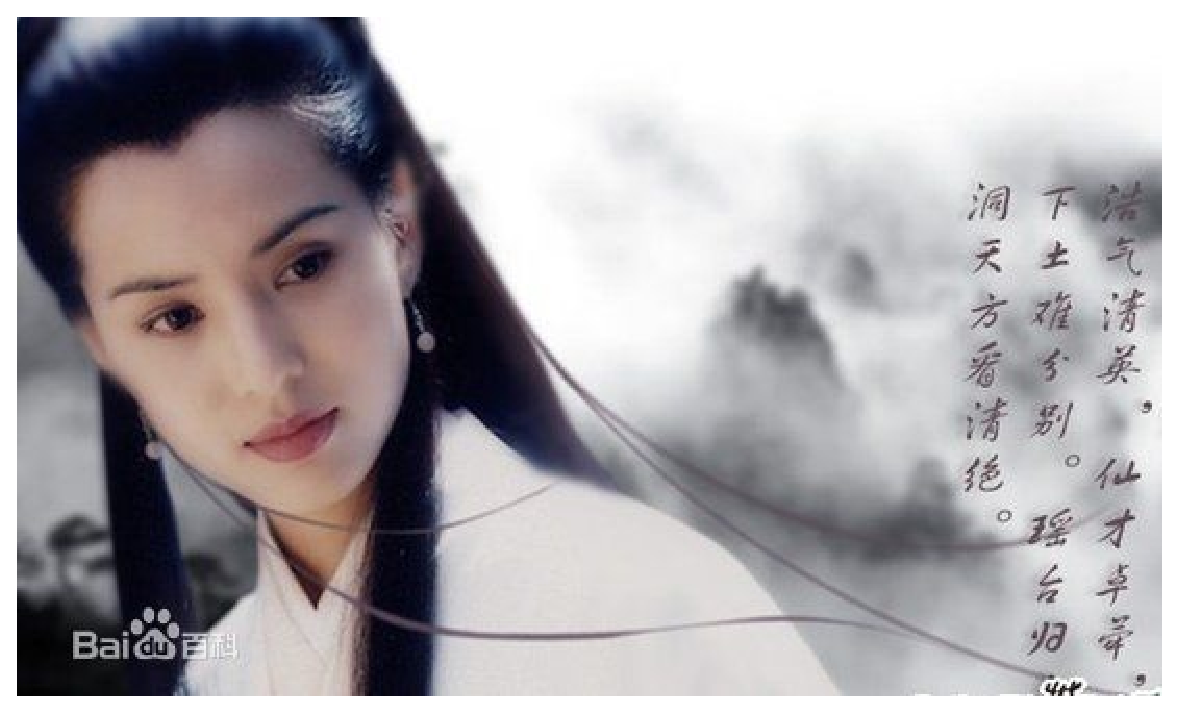
\includegraphics[width=\textwidth]{lrt}
  \caption*{图~321\hskip1em 这是手动编号但不出现索引中的图片例子}
  \label{tab:badfigure3}    
\end{figure}

%%%
%%% End of File
%%%

% \end{appendix}
% 
% % 参考文献
% \bibliographystyle{sdubib}
% \bibliography{ref/kungfu}
% 
% % 致谢
% %%% Local Variables:
%%% mode: latex
%%% TeX-master: "../main"
%%% End:

\chapter{致\hspace{1em}谢}
\echapter{Acknowledgement}

在这里写一些感谢的话。

感谢导师,感谢学科组老师,感谢师兄弟、师姐妹,感谢朋友和家人等等等等等。

感谢学校,感谢社会,感谢教育,感谢国家。好吧。

感谢 \sduthesis{},为我的论文排版节约了大量时间。

感谢王伊蕾师姐提供的学位论文评阅及答辩情况表格代码,和外文论文排版代码,以及对博士论文格式的悉心校对。

%%%
%%% End of File
%%%

% 
% % 攻读学位期间发表的学术论文/参与的科研项目
% \chapter{攻读硕士学位期间完成论文情况}
\echapter{Paper Published}

\begin{enumerate}
    \item \textbf{Guo Jing} and Huang Yaoshi. ``桃花岛花草养殖综述.'' 桃花岛学报, 1250 9th International Conference on. MISC, 1250.
    \item \textbf{Guo Jing} and Hong Qigong. ``降龙十八掌掌法精要.'' 武林学报, 1245 12th International Conference on. KungFu, 1245.
\end{enumerate}


\chapter{攻读学位期间参与科研项目情况}
\echapter{Research Projects Participated}

\begin{enumerate}
    \item 桃花岛导弹防御系统的研究与开发~~桃花岛973项目(No.1244THD10188)
\end{enumerate}

% 
% % 表格、插图、公式索引。带*的版本不生成目录项
% % 山东大学没有索引的要求,Just in case.
% %\listoftables
% %\listoffigures
% %\listofequations*
% 
% \end{document}
% \end{example}
%
% \subsection{选项}
% \label{sec:option}
% 本模板提供了一些选项以方便使用:
% \begin{description}
%
% \item[master]
%   如果写硕士论文将此选项打开。
%   \begin{example}
% \documentclass[master]{sduthesis}
%   \end{example}
%
% \item[doctor]
%   如果写博士论文将此选项打开。
%   \begin{example}
% \documentclass[doctor]{sduthesis}
%   \end{example}
%
% \item[secret]
%   涉秘论文开关。配合另外两个命令 |\secretlevel| 和 |\secretyear| 分别用来指定保
%   密级别和保密时间。可以通过:
%   \cs{secretlevel}|{|绝密|}| 和 \cs{secretyear}|{|10|}| 年独立修改。
%   \begin{example}
% \documentclass[master, secret]{sduthesis}
%   \end{example}
%
% \item[equival,engineer]
%   同等学力或专业学位开关。打开后,会在封面打印``同等学力.../专业学位''字样。
%
% \item[openany, openright]
%   正规出版物的章节出现在奇数页,也就是右手边的页面,这就是 \texttt{openright},
%   也是 \sduthesis 的默认选项。在这种情况下,如果前一章的最后一页也是奇数,那么
%   模板会自动生成一个纯粹的空白页。
%
% \item[dvips,dvipdfm,pdftex,xetex]
%   这些选项主要是配合 \pkg{hyperref} 能正确生成书签和链接,以及所有其它对底层驱动有依
%   赖的包。一般来说,这些选项可以忽略,不过一旦指定了,就要保证使用对应的命令编
%   译,否则模板会报错。
%
%   比如,如果你指定了xetex选项:
% \begin{example}
% \documentclass[doctor,xetex]{sduthesis}
% \end{example}
%   那么,编译时就要使用Xe\LaTeX :
% \begin{shell}
% $ make thesis METHOD=xetex
% \end{shell}
% 其它选项类似,但是dvips例外,因为Makefile默认为dvips方式。
%
% \item[gbk,utf]
%   文档编码。模板默认打开utf。
%
% \item[arial]
%   使用真正的 arial 字体。此选项会装载 arial 字体宏包,如果此宏包不存在,就装
%   载Helvet。arialtoc 和 arialtitle 不受 arial 的影响。因为一般的 \TeX{} 发行都
%   没有 arial 字体,所以默认采用 Helvet,因为二者效果非常相似。如果你执着的要
%   用arial 字体,请参看:\href{http://www.mail-archive.com/ctan-ann@dante.de/msg00627.html}{Arial
%     字体}。
%
% \item[arialtoc]
%  目录项(章目录项除外)中的英文是否用 arial 字体。模板默认关闭。
%
% \item[arialtitle]
%  章节标题中英文是否用 arial 字体。本选项不用用户操心,模板默认打开。
% \end{description}
%
% \subsection{字体配置}
% \label{sec:font-config}
% 正确配置中文字体是使用模板的第一步。模板有两种字体使用方式:
% \begin{itemize}
%   \item 基于传统 CJK 包,使用 latex、pdflatex 编译;
%   \item 基于 xeCJK 包,使用 xelatex 编译。
% \end{itemize}
%
% 第一种方式的字体配置比较繁琐,建议使用 donated 制作的中文字体包(自
% 包含安装方法),请用户自行下载安装,此处不再赘述。
% 
% 本模板推荐使用第二种方法,模板默认采用 Windows 7 的六款字体,配置如下:
% \begin{example}
% \setCJKmainfont[BoldFont={SimHei}, ItalicFont={KaiTi}]{SimSun}
% \setCJKsansfont{SimHei}
% \setCJKmonofont{KaiTi}
% \setCJKfamilyfont{song}{SimSun}
% \setCJKfamilyfont{hei}{SimHei}
% \setCJKfamilyfont{fs}{FangSong}
% \setCJKfamilyfont{kai}{KaiTi}
% \setCJKfamilyfont{li}{LiSu}
% \setCJKfamilyfont{you}{YouYuan}
% \end{example}
%
% 如果你是 Windows XP 用户,按照如下配置:
% \begin{example}
% \setCJKmainfont[BoldFont={SimHei}, ItalicFont={KaiTi}]{SimSun}
% \setCJKsansfont{SimHei}
% \setCJKmonofont{KaiTi_GB2312}
% \setCJKfamilyfont{song}{SimSun}
% \setCJKfamilyfont{hei}{SimHei}
% \setCJKfamilyfont{fs}{FangSong_GB2312}
% \setCJKfamilyfont{kai}{KaiTi_GB2312}
% \setCJKfamilyfont{li}{LiSu}
% \setCJKfamilyfont{you}{YouYuan}
% \end{example}
%
% 当然,你也可以选择Adobe的四款(宋、仿宋、黑体、楷体)免费字体,但是大多数系统中都没有默认安装,
% 用户需要自行下载并把字体放入系统字体文件夹(也可以指定自定义文件夹):
% \begin{example}
% \setCJKmainfont[BoldFont={Adobe Heiti Std}, ItalicFont={Adobe Kaiti Std}]%
%    {Adobe Song Std}
% \setCJKsansfont{Adobe Heiti Std}
% \setCJKmonofont{Adobe Kaiti Std}
% \setCJKfamilyfont{song}{Adobe Song Std}
% \setCJKfamilyfont{hei}{Adobe Heiti Std}
% \setCJKfamilyfont{fs}{Adobe Fangsong Std}
% \setCJKfamilyfont{kai}{Adobe Kaiti Std}
% \setCJKfamilyfont{li}{Adobe Kaiti Std} % TODO: 用隶书字体代替
% \setCJKfamilyfont{you}{Adobe Kaiti Std} % TODO: 用幼圆字体代替
% \end{example}
%
% 总而言之,用户可以通过命令:
% \begin{shell}
% $ fc-list -f "%{family}\n" : lang=zh
% \end{shell}
%
% 来查看系统中现有的中文字体,并相应替换上述配置。
%
% \subsection{命令}
% \label{sec:command}
% 模板中的命令分为两类:一是格式控制,二是内容替换。格式控制如字体、字号、字距和
% 行距。内容替换如姓名、院系、专业、导师等等。其中内容替换命令居多,而且主要集中
% 在封面上。首先来看格式控制命令。
%
% \subsubsection{基本控制命令}
% \label{sec:basiccom}
%
% \myentry{字体}
% \DescribeMacro{\song}
% \DescribeMacro{\fs}
% \DescribeMacro{\hei}
% \DescribeMacro{\kai}
% \DescribeMacro{\li}
% \DescribeMacro{\you}
% 等分别用来切换宋体、仿宋、黑体、楷体、隶书和幼圆字体。为了兼容不同用户的习惯,模
% 板还定义了另外一些字体切换命令,对应关系如下:
%
% \begin{center}
% \begin{tabular}{llllll}\hline
%  \cs{song} &\cs{fs}&\cs{hei}&\cs{kai}&\cs{li}&\cs{you}\\\hline
%  \cs{songti}&\cs{fangsong}&\cs{heiti}&\cs{kaishu}&\cs{lishu}&\cs{youyuan}\\\hline
% \end{tabular}
% \end{center}
%
% \begin{example}
% {\song 乾:元,亨,利贞}
% {\fs 初九,潜龙勿用}
% {\hei 九二,见龙在田,利见大人}
% {\kai 九三,君子终日乾乾,夕惕若,厉,无咎}
% {\li 九四,或跃在渊,无咎}
% {\hei 九五,飞龙在天,利见大人}
% {\song 上九,亢龙有悔}
% {\you 用九,见群龙无首,吉}
% \end{example}
%
% \myentry{字号}
% \DescribeMacro{\chuhao}
% 等命令定义一组字体大小,分别为:
%
% \begin{center}
% \begin{tabular}{lllll}
% \hline
% |\chuhao|&|\xiaochu|&|\yihao|&|\xiaoyi| &\\
% |\erhao|&|\xiaoer|&|\sanhao|&|\xiaosan|&\\
% |\sihao|& |\banxiaosi|&|\xiaosi|&|\dawu|&|\wuhao|\\
% |\xiaowu|&|\liuhao|&|\xiaoliu|&|\qihao|& |\bahao|\\\hline
% \end{tabular}
% \end{center}
%
% 使用方法为:\cs{command}\oarg{num},其中 |command| 为字号命令,|num| 为行距。比
% 如 |\xiaosi[1.5]| 表示选择小四字体,行距 1.5 倍。
%
% \begin{example}
% {\erhao 二号 \sanhao 三号 \sihao 四号  \qihao 七号}
% \end{example}
%
% \myentry{字距}
% \DescribeMacro{\ziju}
% 更改汉字之间默认的距离,使用格式为 |\ziju{4bp}|,其中的距离只要是合格的 \TeX{} 距离即可。
%
% \myentry{密级}
% \DescribeMacro{\secretlevel}
% \DescribeMacro{\secretyear}
% 定义秘密级别和年限(注意:这两个命令只有在打开secret选项时才生效):
%   \begin{example}
% \secretyear{5}
% \secretlevel{内部}
%   \end{example}
%
% \myentry{引用方式}
% \DescribeMacro{\onlinecite}

% 学校要求的参考文献引用有两种模式:(1)上标模式。比如``同样的工作有很
% 多$^{[1,2]}$\ldots''。(2)正文模式。比如``文献[3] 中详细说明了\ldots''。其中上标
% 模式使用远比正文模式频繁,所以为了符合使用习惯,上标模式仍然用常规
% 的 |\cite{key}|,而 |\onlinecite{key}| 则用来生成正文模式。
%
% 关于参考文献模板推荐使用 BIB\TeX,关于中文参考文献需要额外增加一个 Entry: lang,将其设置为 \texttt{zh}
% 用来指示此参考文献为中文,以便 sdubib.bst 处理。如:
% \begin{example}
% @INPROCEEDINGS{cnproceed,
%   author    = {王重阳 and 黄药师 and 欧阳峰 and 洪七公 and 段皇帝},
%   title     = {武林高手从入门到精通},
%   booktitle = {第~$N$~次华山论剑},
%   year      = 2006,
%   address   = {西安, 中国},
%   month     = sep,
%   lang      = "zh",
% }
%
% @ARTICLE{cnarticle,
%   AUTHOR  = "贾宝玉 and 林黛玉 and 薛宝钗 and 贾探春",
%   TITLE   = "论刘姥姥食量大如牛之现实意义",
%   JOURNAL = "红楼梦杂谈",
%   PAGES   = "260--266",
%   VOLUME  = "224",
%   YEAR    = "1800",
%   LANG    = "zh",
% }
% \end{example}
%
% \myentry{破折号}
% \DescribeMacro{\pozhehao}
% 中文破折号在 CJK-\LaTeX\ 里没有很好的处理,我们平时输入的都是两个小短线,比如这
% 样,{\hei 中国——中华人民共和国}。这不符合中文习惯。所以这里定义了一个命令生成更
% 好看的破折号,不过这似乎不是一个好的解决办法。有同学说不能用在 |\section| 等命
% 令中使用,简单的办法是可以提供一个不带破折号的段标题:\cs{section}\oarg{没有破
%   折号精简标题}\marg{带破折号的标题}。
%
%
% \subsubsection{封面命令}
% \label{sec:titlepage}
% 下面是内容替换命令,其中以 |c| 开头的命令跟中文相关,|e| 开头则为对应的英文。
% 这部分的命令数目比较多,但实际上都相当简单,套用即可。
%
% 大多数命令的使用方法都是: \cs{command}\marg{arg},例外者将具体指出。这些命令都
% 在示例文档的 data/cover.tex 中。
%
% \myentry{论文标题}
% \DescribeMacro{\ctitle}
% \DescribeMacro{\etitle}
% \begin{example}
% \ctitle{论文中文题目}
% \etitle{Thesis English Title}
% \end{example}
%
% \myentry{作者姓名}
% \DescribeMacro{\cauthor}
% \DescribeMacro{\eauthor}
% \begin{example}
% \cauthor{中文姓名}
% \eauthor{Your name in PinYin}
% \end{example}
%
% \myentry{院系名称}
% \DescribeMacro{\cdepartment}
% \DescribeMacro{\edepartment}
%
% \begin{example}
% \cdepartment{系名全称}
% \edepartment{Department name in English}
% \end{example}
%
% \myentry{专业名称}
% \DescribeMacro{\cmajor}
% \DescribeMacro{\emajor}
% \begin{example}
% \cmajor{专业名称}
% \emajor{Major in English}
% \end{example}
%
% \myentry{导师姓名}
% \DescribeMacro{\csupervisor}
% \DescribeMacro{\esupervisor}
% \begin{example}
% \csupervisor{导师~教授}
% \esupervisor{Supervisor}
% \end{example}
%
% \myentry{合作导师}
% \DescribeMacro{\ccosupervisor}
% \DescribeMacro{\ecosupervisor}
% \begin{example}
% \ccosupervisor{合作导师~教授}
% \ecosupervisor{Tiny Boss}
% \end{example}
%
% \myentry{论文成文日期}
% \DescribeMacro{\cdate}
% \DescribeMacro{\edate}
% 默认为当前时间,也可以自己指定。
% \begin{example}
% \cdate{中文日期}
% \edate{English Date}
% \end{example}
%
% \myentry{封面其它参数}
% \DescribeMacro{\catalognumber}
% \DescribeMacro{\schoolnumber}
% \DescribeMacro{\studentnumber}
% 分别代表分类号,单位代码和学号
% \begin{example}
% \catalognumber{TP393}
% \schoolnumber{10422}
% \studentnumer{20145501942}
% \end{example}
%
% \subsubsection{章节与目录}
% \label{sec:chapandtoc}
% \myentry{章节与目录}
% \DescribeMacro{\echapter}
% \DescribeMacro{\esection}
% \DescribeMacro{\chapter}
% \DescribeMacro{\section}
% \DescribeMacro{\tableofecontents}
% 山东大学有英文目录的要求,我们定义了一系列带 e 的命令用于生成英文目录。
% 带 e 的版本只生成目录项,不会生成实际的标题。原始命令(不带 e 的),如果
% 标题前面有空的方括号,则只生成标题,不产生目录项。
% \begin{example}
% \chapter{这是一普通的章标题}
% \chapter[]{本章不会出现在目录中}
% \echapter{Chapter Title in English}
% % 还有\esection, \esubsection 等都类似。
% \tableofecontents% 生成英文目录,放在合适的位置
% \end{example}
%
% \subsubsection{其它部分}
% \label{sec:otherparts}
% 论文其它主要部分命令:
%
% \myentry{符号对照表}
% \DescribeEnv{denotation}
% 主要符号表环境。简单定义的一个 list,跟 description 非常类似,使用方法参见示例
% 文件。带一个可选参数,用来指定符号列的宽度(默认为 2.5cm)。
% \begin{example}
% \begin{denotation}
%   \item[E] 能量
%   \item[m] 质量
%   \item[c] 光速
% \end{denotation}
% \end{example}
%
% 如果你觉得符号列的宽度不满意,那可以这样来调整:
% \begin{example}
% \begin{denotation}[1.5cm] % 设置为 1.5cm
%   \item[E] 能量
%   \item[m] 质量
%   \item[c] 光速
% \end{denotation}
% \end{example}
%
% \myentry{索引}
% 山东大学并没有索引的要求,模板提供这三条命令只是以防万一。
%
% 插图、表格和公式三个索引命令分别如下,将其插入到期望的位置即可(带星号的命令表
% 示对应的索引表不会出现在目录中):
%
% \begin{center}
% \begin{tabular}{ll}
% \hline
%   {\hei 命令} & {\hei 说明} \\\hline
% \cs{listoffigures} & 插图索引\\
% \cs{listoffigures*} & \\\hline
% \cs{listoftables} & 表格索引\\
% \cs{listoftables*} & \\\hline
% \cs{listofequations} & 公式索引\\
% \cs{listofequations*} & \\\hline
% \end{tabular}
% \end{center}
%
% \LaTeX{} 默认支持插图和表格索引,是通过 \cs{caption} 命令完成的,因此它们必须出
% 现在浮动环境中,否则不被计数。
%
% 公式索引为本模板扩展,模板扩展了 \pkg{amsmath} 几个内部命令,使得公式编号样式和
% 自动索引功能非常方便。一般来说,你用到的所有数学环境编号都没问题了,这个可以参
% 看示例文档。如果你有个非常特殊的数学环境需要加入公式索引,那么请使
% 用 \cs{equcaption}\marg{编号}。此命令表示 equation caption,带一个参数,即显示
% 在索引中的编号。因为公式与图表不同,我们很少给一个公式附加一个标题,之所以起这
% 么个名字是因为图表就是通过 \cs{caption} 加入索引的,\cs{equcaption} 完全就是为
% 了生成公式列表,不产生什么标题。
%
% 使用方法如下。假如有一个非 equation 数学环境 mymath,只要在其中写一
% 句 \cs{equcaption} 就可以将它加入公式列表。
% \begin{example}
% \begin{mymath}
%   \label{eq:emc2}\equcaption{\ref{eq:emc2}}
%   E=mc^2
% \end{mymath}
% \end{example}
%
% 当然 mymath 正文中公式的编号需要你自己来做。
%
% 同图表一样,附录中的公式有时候也不希望它跟全文统一编号,而且不希望它出现在公式
% 索引中,目前的解决办法就是利用 \cs{tag*}\marg{公式编号} 来解决。用法很简单,此
% 处不再罗嗦,实例请参看示例文档附录 A 的第一个公式。
%
% \myentry{附录}
% \DescribeEnv{appendix}
% 所有的附录都插到这里来。因为附录会更改默认的 chapter 属性,而且和前面和后面的都不一样,
% 所以实现为环境可以保证全局的属性不受影响。
% \begin{example}
% \begin{appendix}
%  %%% Local Variables: 
%%% mode: latex
%%% TeX-master: "../main"
%%% End: 

\chapter{特殊浮动对象}
\echapter{Special Float Object}
\label{cha:speobj}
如果附录中的公式不想让它出现在公式索引中,那就请用 \verb|\tag*{xxx}|

\begin{equation}\tag*{(123)} 
\left\{\begin{array}{l}
\max \,\,f(x)\\[0.1 cm]
\mbox{subject to:} \\ [0.1 cm]
\qquad g_j(x)\le 0,\quad j=1,2,\cdots,p
\end{array}\right.
\end{equation}

\begin{table}[ht]
  \centering
  \caption*{Table~111\hskip1em This is an example for manually numbered table, which
    would not appear in the list of tables}
  \label{tab:badtabular2}
  \begin{tabular}[c]{|c|m{0.8in}|c|c|c|c|c|}\hline
    \multicolumn{2}{|c|}{Network Topology} & \# of nodes & 
    \multicolumn{3}{c|}{\# of clients} & Server \\\hline
    GT-ITM & Waxman Transit-Stub & 600 &
    \multirow{2}{2em}{2\%}& 
    \multirow{2}{2em}{10\%}& 
    \multirow{2}{2em}{50\%}& 
    \multirow{2}{1.2in}{Max. Connectivity}\\\cline{1-3}
    \multicolumn{2}{|c|}{Inet-2.1} & 6000 & & & &\\\hline
    \multirow{2}{1in}{blahblah} & jin  & jin &\multicolumn{4}{c|}{\multirow{2}*{\sduthesis}}\\\cline{2-3}
    & \multicolumn{2}{c|}{ABCDEF} &\multicolumn{4}{c|}{} \\\hline
\end{tabular}  
\end{table}

\begin{figure}[h]
  \centering
  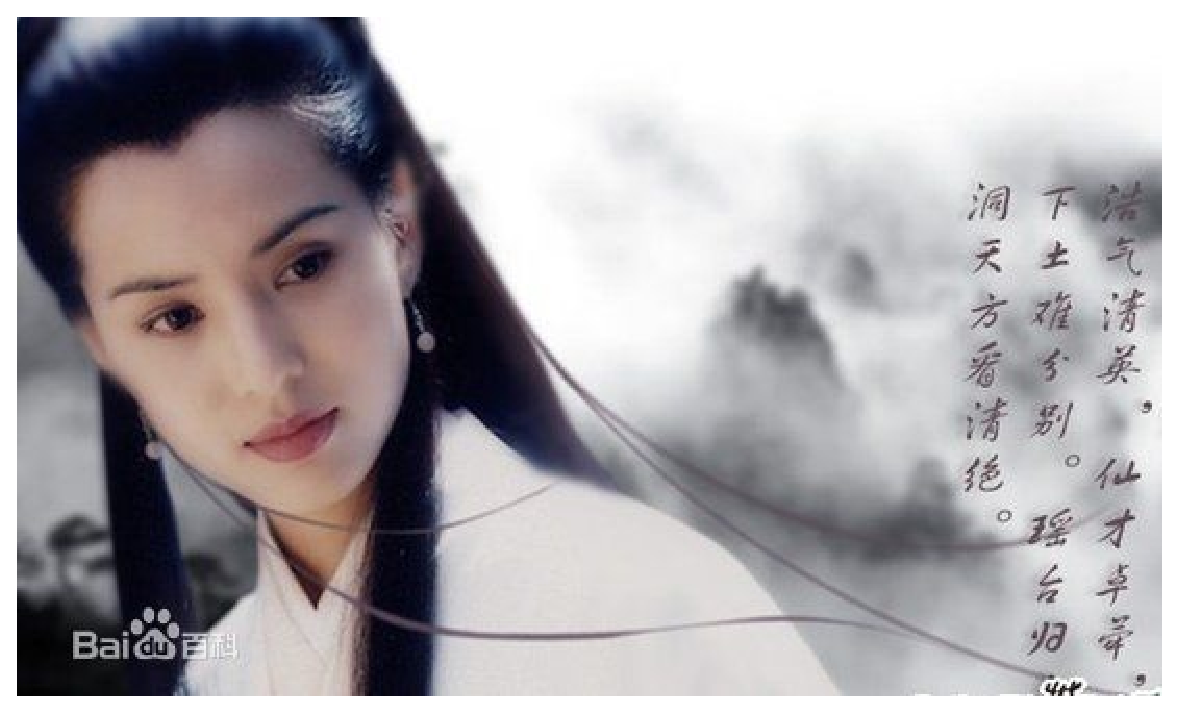
\includegraphics[width=\textwidth]{lrt}
  \caption*{Figure~123\hskip1em This is an example for manually numbered figure,
    which would not appear in the list of figures}
  \label{tab:badfigure2}    
\end{figure}

\begin{table}[ht]
\centering
  \centering
  \caption*{表~222\hskip1em 这是手动编号但不出现在索引中的表格例子}
  \label{tab:badtabular3}
  \begin{tabular}[c]{|c|m{0.8in}|c|c|c|c|c|}\hline
    \multicolumn{2}{|c|}{Network Topology} & \# of nodes & 
    \multicolumn{3}{c|}{\# of clients} & Server \\\hline
    GT-ITM & Waxman Transit-Stub & 600 &
    \multirow{2}{2em}{2\%}& 
    \multirow{2}{2em}{10\%}& 
    \multirow{2}{2em}{50\%}& 
    \multirow{2}{1.2in}{Max. Connectivity}\\\cline{1-3}
    \multicolumn{2}{|c|}{Inet-2.1} & 6000 & & & &\\\hline
    \multirow{2}{1in}{blah} & blah  & jin &\multicolumn{4}{c|}{\multirow{2}*{\sduthesis}}\\\cline{2-3}
    & \multicolumn{2}{c|}{ABCDEF} &\multicolumn{4}{c|}{} \\\hline
\end{tabular}  
\end{table}

\begin{figure}[!htbp]
  \centering
  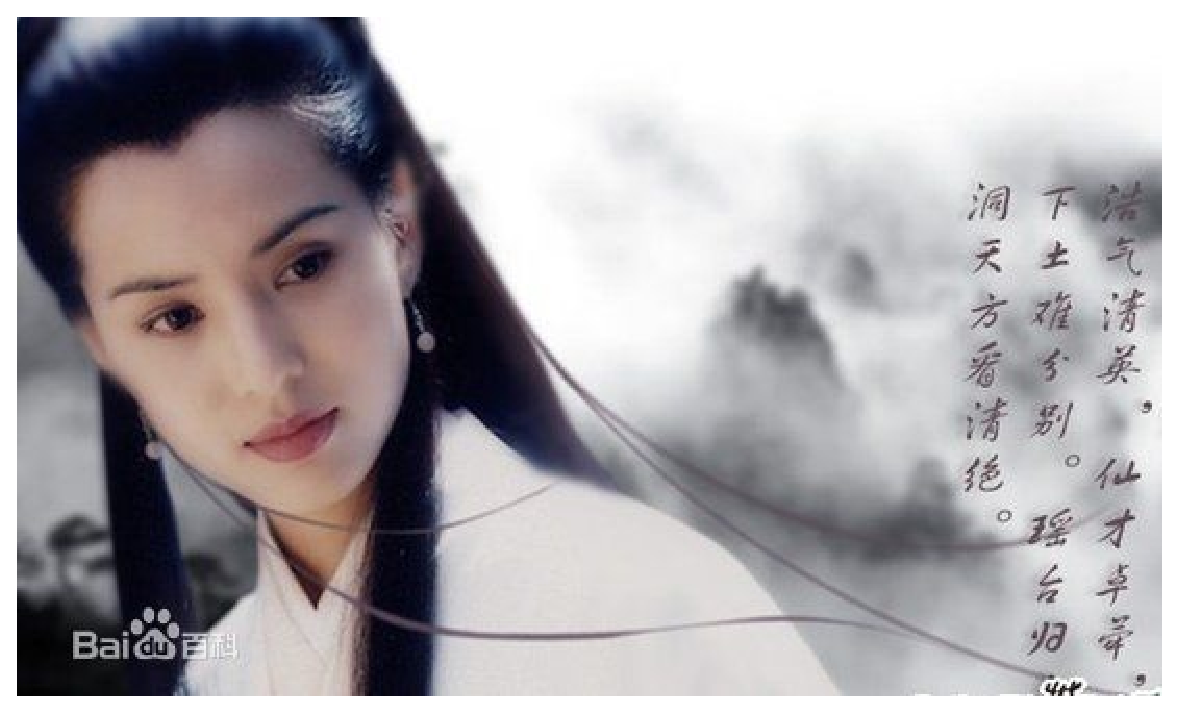
\includegraphics[width=\textwidth]{lrt}
  \caption*{图~321\hskip1em 这是手动编号但不出现索引中的图片例子}
  \label{tab:badfigure3}    
\end{figure}

%%%
%%% End of File
%%%

%  \chapter{逍遥游}
\echapter{Xiao Yao You}

北冥(míng)有鱼,其名为鲲(kūn)。鲲之大,不知其几千里也。化而为鸟,其名为鹏。鹏之背,不知其几千里也;怒而飞,其翼若垂天之云。是鸟也,海运则将徙(xǐ)于南冥。南冥者,天
池也。齐谐者,志怪者也。谐之言曰:“鹏之徙于南冥也,水击三千里,抟(tuán)扶摇而上者九万里,去以六月息者也。”野马也,尘埃也,生物之以息相吹也。天之苍苍,其正色邪(yé)?其远
而无所至极邪?其视下也,亦若是则已矣。且夫水之积也不厚,则其负大舟也无力。覆杯水于坳(ào)堂之上,则芥(jiè)为之舟,置杯焉则胶,水浅而舟大也。风之积也不厚,则其负大翼也
无力。故九万里,则风斯在下矣,而后乃今培风;背负青天,而莫之夭阏(yāo è)者,而后乃今将图南。蜩(tiáo)与学鸠笑之曰:“我决(xuè)起而飞,抢(qiāng)榆枋(fāng),时则不至,
而控于地而已矣,奚以之九万里而南为?”适莽(mǎng)苍者,三餐而反,腹犹果然;适百里者,宿(xiu)舂(chōng)粮;适千里者,三月聚粮。之二虫又何知!

小知(zhì)不及大知(32),小年不及大年。奚以知其然也?朝(zhāo)菌(jūn)不知晦朔(huì shuò),蟪蛄不知春秋,此小年也。楚之南有冥灵者,以五百岁为春,五百岁为秋;上古有大椿
(chūn)者,以八千岁为春,八千岁为秋,此大年也。而彭祖乃今以久特闻,众人匹之,不亦悲乎!汤之问棘也是已。(汤问棘曰:‘上下四方有极乎?’棘曰:'无极之外复无极也。【注】)穷发
(fà)之北,有冥海者,天池也。有鱼焉,其广数千里,未有知其修者,其名为鲲。有鸟焉,其名为鹏,背若泰山,翼若垂天之云,抟扶摇羊角而上者九万里,绝云气,负青天,然后图南,且适
南冥也。斥鴳(yàn)笑之曰:‘彼且奚适也?我腾跃而上,不过数仞而下,翱翔蓬蒿之间,此亦飞之至也。而彼且奚适也?’”此小大之辩也。

故夫知(zhì)效一官,行比一乡,德合一君,而(néng)征一国者,其自视也亦若此矣。而宋荣子犹然笑之。且举世而誉之而不加劝,举世而非之而不加沮(jǔ),定乎内外之分,辩乎荣辱之境,
斯已矣。彼其于世,未数(shuò)数(shuò)然也。虽然,犹有未树也。夫列子御风而行,泠(líng)然善也,旬有(yòu)五日而后反。彼于致福者,未数数然也。此虽免乎行,犹有所待者也。
若夫乘天地之正,而御六气之辩,以游无穷者,彼且恶乎待哉?故曰:至人无己,神人无功,圣人无名。


% \end{appendix}
% \end{example}
%
% \myentry{列表环境}
% \DescribeEnv{itemize}
% \DescribeEnv{enumerate}
% \DescribeEnv{description}
% 为了适合中文习惯,模板将这三个常用的列表环境用 \pkg{paralist} 对应的压缩环境替
% 换。一方面满足了多余空间的清楚,另一方面可以自己指定标签的样式和符号。细节请参
% 看 \pkg{paralist} 文档,此处不再赘述。
%
% \subsection{数学环境}
% \label{sec:math}
% \sduthesis{} 定义了常用的数学环境:
%
% \begin{center}
% \begin{tabular}{*{7}{l}}\hline
%   axiom & theorem & definition & proposition & lemma & conjecture &\\
%   公理 & 定理 & 定义 & 命题 & 引理 & 猜想 &\\\hline
%   proof & corollary & example & exercise & assumption & remark & problem \\
%   证明 & 推论 & 例子& 练习 & 假设 & 注释 & 问题\\\hline
% \end{tabular}
% \end{center}
%
% 比如:
% \begin{example}
% \begin{definition}
% 道千乘之国,敬事而信,节用而爱人,使民以时。
% \end{definition}
% \end{example}
% 产生(自动编号):\\[5pt]
% \fbox{{\hei 定义~1.1~~~} {道千乘之国,敬事而信,节用而爱人,使民以时。}}
%
% 列举出来的数学环境毕竟是有限的,如果想用{\hei 胡说}这样的数学环境,那么很容易定义:
% \begin{example}
% \newtheorem{nonsense}{胡说}[chapter]
% \end{example}
%
% 然后这样使用:
% \begin{example}
% \begin{nonsense}
% 契丹武士要来中原夺武林秘笈。\pozhehao 慕容博
% \end{nonsense}
% \end{example}
% 产生(自动编号):\\[5pt]
% \fbox{{\hei 胡说~1.1~~~} {契丹武士要来中原夺武林秘笈。\kern0.3ex\rule[0.8ex]{2em}{0.1ex}\kern0.3ex 慕容博}}
% 
% \subsection{关于查重版本}
% Makefile的默认编译方式生成的pdf文件不支持拷贝(拷贝出来是乱码),影响查重。一个直接的解决方法是使用pdf\LaTeX 编译:
% \begin{shell}
% $ make thesis METHOD=pdftex
% \end{shell}
% 或者手动执行:
% \begin{shell}
% $ pdflatex main.tex
% $ bibtex main
% $ pdflatex main.tex
% $ pdflatex main.tex
% \end{shell}
%
% \subsection{自定义以及其它}
% \label{sec:othercmd}
% 模板的配置文件 sduthesis.cfg 中定义了很多固定词汇,一般无须修改。如果有特殊需求,两种修改方法:
% 一、在 sduthesis.cfg中直接修改,但是模板升级后会覆盖修改;二、在 main.tex 导言区修改。
%
% \subsection{Q \& A}
% \label{sec:qanda}
% \begin{enumerate}
%   \item 为什么使用默认编译方式,生成的pdf文件汉字不显示? \\
%         这是因为字体配置问题。如果你使用CTeX,需要运行CTeX-FontSetup.exe:安装过程中勾选
%         从TTC中提取TTF,生成TFM文件,生成Type1字库,使用Type1字库,和所有可用字体即可。 \\
%   \item 使用Xe\LaTeX 编译,出现The usyr source file could not be found 和 PK font usyr could
%         not be found 错误? \\
%         Sorry! 我也不知道怎么回事。大概和字体设置有关。欢迎懂Xe\LaTeX 的同学补充。
% \end{enumerate}
%
%
% \section{致谢}
% \label{sec:thanks}
% 感谢清华大学薛瑞尼老师撰写的 \thuthesis{} 和 thuthesis.pdf,\sduthesis{} 完全继承自 \thuthesis{},做了``山大化''处理,而 sduthesis.pdf(本文档)完全从 thuthesis.pdf 修改而来。
% 
% 本模板全力支持硕士论文;本模板想要支持博士论文,但目前还没有博士使用过,很多格式都没有和规范比对;本模板不想要支持博士后出站报告,因为目标用户太少;本模板拒绝支持本科论文,因为已有另一个Github项目存在。
%
% 本人马上就要离开山东大学,硕士学位论文即是用此模板完成的。毕业后,本人维护此模板的时间和精力必然非常有限,希望有志于此的山大人能够接手维护下去,为同学服务。
%
% 最后,感谢密码学与信息安全实验室提供的自由、平等、健康的学术与学习环境,感谢在精神上支持本项目的朋友,你们的鼓励也是我的动力之一。
%
% 
% \StopEventually{\PrintIndex}%
% \clearpage
%
% \section{实现细节}
%
% \subsection{基本信息}
%    \begin{macrocode}
%<cls>\NeedsTeXFormat{LaTeX2e}[1999/12/01]
%<cls>\ProvidesClass{sduthesis}
%<cfg>\ProvidesFile{sduthesis.cfg}
%<cls|cfg>[2014/05/05 0.1.0 Shandong University Thesis Template]
%    \end{macrocode}
%
% \subsection{定义选项}
% \label{sec:defoption}
% TODO: 所有的选项用 \pkg{xkeyval} 来重构,现在的太罗唆了。
%
% 定义文档所使用编码
%    \begin{macrocode}
%<*cls>
\newif\ifsdu@UTF
\newif\ifsdu@GBK
\DeclareOption{utf}{\sdu@UTFtrue\sdu@GBKfalse}
\DeclareOption{gbk}{\sdu@GBKtrue\sdu@UTFfalse}
%    \end{macrocode}
%
% 定义论文类型以及是否涉密
%    \begin{macrocode}
\hyphenation{Sdu-Thesis}
\def\sduthesis{\textsc{SduThesis}}
\def\version{0.1.0}
\newif\ifsdu@master\sdu@masterfalse
\newif\ifsdu@doctor\sdu@doctorfalse
\newif\ifsdu@secret\sdu@secretfalse
\DeclareOption{master}{\sdu@mastertrue}
\DeclareOption{doctor}{\sdu@doctortrue}
\DeclareOption{secret}{\sdu@secrettrue}
%    \end{macrocode}
%
% 是否同等学力和专业学位
%    \begin{macrocode}
\newif\ifsdu@equival\sdu@equivalfalse
\newif\ifsdu@engineer\sdu@engineerfalse
\DeclareOption{equival}{\sdu@equivaltrue}
\DeclareOption{engineer}{\sdu@engineertrue}
%    \end{macrocode}
%
% 使用 dvips,dvipdfm, pdflatex 还是 xelatex
%    \begin{macrocode}
\newif\ifsdu@dvips
\newif\ifsdu@dvipdfm
\newif\ifsdu@xetex
\newif\ifsdu@pdftex
\DeclareOption{dvips}{\sdu@dvipstrue}
\DeclareOption{dvipdfm}{\sdu@dvipdfmtrue}
\DeclareOption{pdftex}{\sdu@pdftextrue}
\DeclareOption{xetex}{\sdu@xetextrue}
%    \end{macrocode}
%
% 如果需要使用 arial 字体,请打开 [arial] 选项
%    \begin{macrocode}
\newif\ifsdu@arial
\DeclareOption{arial}{\sdu@arialtrue}
%    \end{macrocode}
%
% 目录中英文是否用 arial
%    \begin{macrocode}
\newif\ifsdu@arialtoc
\DeclareOption{arialtoc}{\sdu@arialtoctrue}
%    \end{macrocode}
% 章节标题中的英文是否用 arial
%    \begin{macrocode}
\newif\ifsdu@arialtitle
\DeclareOption{arialtitle}{\sdu@arialtitletrue}
%    \end{macrocode}
%
% 将选项传递给 book 类
%    \begin{macrocode}
\DeclareOption*{\PassOptionsToClass{\CurrentOption}{book}}
%    \end{macrocode}
%
% \cs{ExecuteOptions} 的参数之间用逗号分割,不能有空格。开始不知道,折腾了老半
% 天。
%    \begin{macrocode}
\ExecuteOptions{utf,arialtitle}
\ProcessOptions\relax
\LoadClass[12pt,a4paper]{book}
%    \end{macrocode}
%
% 用户至少要提供一个选项:指定论文类型。
%    \begin{macrocode}
\ifsdu@master\relax\else
  \ifsdu@doctor\relax\else
      \ClassError{sduthesis}%
           {You have to specify one of thesis options: master or doctor.}{}
  \fi
\fi
%    \end{macrocode}
%
% 检查用户指定的选项和实际编译命令是否冲突。
%    \begin{macrocode}
\RequirePackage{ifpdf,ifxetex}
\ifsdu@xetex\RequireXeTeX\fi
\def\RequirePDFTeX{%
  \ifpdf\else
    \ClassError{sduthesis}%
               {pdfLaTeX is required to compile this document!}{}
  \fi}
\ifsdu@pdftex\RequirePDFTeX\fi
\def\sdu@checkoption#1#2{%
  \@for\reserved@a:=#2\do{%
    \csname ifsdu@\reserved@a\endcsname
      \ClassError{sduthesis}%
                 {Please remove `\reserved@a' option when you run #1.}{}
    \fi}}
\ifpdf\sdu@checkoption{pdflatex}{dvips,dvipdfm,xetex}\sdu@pdftextrue\fi%
% force the option to be true
\ifxetex\sdu@checkoption{xelatex}{dvips,dvipdfm,pdftex}\sdu@xetextrue\fi
%    \end{macrocode}
%
%
% \subsection{装载宏包}
% \label{sec:loadpackage}
%
% 引用的宏包和相应的定义。
%    \begin{macrocode}
\RequirePackage{ifthen,calc}
%    \end{macrocode}
%
% \AmSTeX{} 宏包,用来排出更加漂亮的公式。
%    \begin{macrocode}
\RequirePackage{amsmath,amssymb}
%    \end{macrocode}
%
% 用很爽的 \pkg{txfonts} 替换 \pkg{mathptmx} 宏包,同时用它自带的 typewriter 字
% 体替换 courier。必须出现在 \AmSTeX{} 之后。
%    \begin{macrocode}
\RequirePackage{txfonts}
%    \end{macrocode}
%
% 图形支持宏包。
%    \begin{macrocode}
\RequirePackage{graphicx}
%    \end{macrocode}
%
% 并排图形。\pkg{subfigure} 已经不再推荐,用新的 \pkg{subfig}。加入 |config| 选项
% 以便兼容 \pkg{subfigure} 的命令。浮动图形和表格标题样式。\pkg{caption2} 已经不
% 推荐使用,采用新的 \pkg{caption}。它会自动被 \pkg{subfig} 装载进来。所以可以在
% 后面看到 \cs{captionsetup} 的命令。
%    \begin{macrocode}
\RequirePackage[config]{subfig}
%    \end{macrocode}
%
% 首行缩进宏包
%    \begin{macrocode}
\RequirePackage{indentfirst}
%    \end{macrocode}
%
% 更好的列表环境。newitem和newenum选项默认是打开的。
%    \begin{macrocode}
\RequirePackage[neverdecrease]{paralist}
%    \end{macrocode}
%
% 中文支持宏包。XeTeX 模式下直接调用 \pkg{xeCJK},一切问题都搞定了。
%    \begin{macrocode}
\ifsdu@xetex
  \RequirePackage{mathptmx}
% fontspec conflicts with txfonts now, so we have to load other times-math fonts.
  \RequirePackage{xltxtra}
  \RequirePackage[CJKnumber,BoldFont,normalindentfirst]{xeCJK}%,ItalicFont
  \punctstyle{quanjiao}
  % todo: minor fix of CJKnumb
  \def\CJK@null{\kern\CJKnullspace\Unicode{48}{7}\kern\CJKnullspace}
  \defaultfontfeatures{Mapping=tex-text} % use TeX --
%    \end{macrocode}
% 默认采用 Windows 7 的六款 (宋,黑,楷,仿宋,隶书,幼圆) 字体。
%    \begin{macrocode}
\setCJKmainfont[BoldFont={SimHei}, ItalicFont={KaiTi}]{SimSun}
\setCJKsansfont{SimHei}
\setCJKmonofont{KaiTi}% KaiTi_GB2312 for windows XP
\setCJKfamilyfont{song}{SimSun}
\setCJKfamilyfont{hei}{SimHei}
\setCJKfamilyfont{fs}{FangSong}% FangSong_GB2312 for windows XP
\setCJKfamilyfont{kai}{KaiTi}% KaiTi_GB2312 for windows XP
\setCJKfamilyfont{li}{LiSu}
\setCJKfamilyfont{you}{YouYuan}

  \setmainfont{Times New Roman}
  \setsansfont{Arial}
  \setmonofont{Courier New}
%    \end{macrocode}
% 对于 \LaTeX\ 和 PDF\LaTeX,调用 \pkg{CJK} 以及相关的包。注意:\pkg{CJKpunct} 必
% 须放在 \pkg{CJKspace} 之前。
%    \begin{macrocode}
\else
  \RequirePackage{CJKutf8}
  \RequirePackage{CJKnumb}
  \ifsdu@GBK % CJKpunct 在 UTF 下工作的不好。
    \IfFileExists{CJKpunct.sty}%
                 {\RequirePackage{CJKpunct}}%
                 {\ClassWarning{sduthesis}{no CJKpunct.sty availiable!}}
  \fi
  \RequirePackage{CJKspace}
%    \end{macrocode}
% arial 字体需要单独安装,如果不使用 arial 字体,可以用 helvet 字体 |\textsf|
% 模拟,二者基本没有差别。
%    \begin{macrocode}
  \ifsdu@arial
    \IfFileExists{arial.sty}%
                 {\RequirePackage{arial}}%
                 {\ClassWarning{sduthesis}{no arial.sty availiable!}}
  \fi
\fi
%    \end{macrocode}
%
% 可拷贝的 PDF (\pkg{ccmap} 结合 \texttt{pdflatex} 和 \texttt{dvipdfmx} 使用)
%    \begin{macrocode}
\ifsdu@dvips\else
  \ifsdu@xetex\else
    \RequirePackage{ccmap}
  \fi
\fi
%    \end{macrocode}
%
% 定理类环境宏包,其中 \pkg{amsmath} 选项用来兼容 \AmSTeX{} 的宏包
%    \begin{macrocode}
\RequirePackage[amsmath,thmmarks,hyperref]{ntheorem}
%    \end{macrocode}
%
% 表格控制
%    \begin{macrocode}
\RequirePackage{array}
\RequirePackage{longtable}
%    \end{macrocode}
%
% 使用三线表:\cs{toprule},\cs{midrule},\cs{bottomrule}。
%    \begin{macrocode}
\RequirePackage{booktabs}
%    \end{macrocode}
%
% 参考文献引用宏包。
%    \begin{macrocode}
\RequirePackage[numbers,super,sort&compress]{natbib}
%    \end{macrocode}
%
% 生成有书签的 pdf 及其开关,如果你的源文件是gbk编码,请结合 gbk2uni 避免书签乱码。
%    \begin{macrocode}
\RequirePackage{hyperref}
\ifxetex
  \hypersetup{%
    CJKbookmarks=true}
\else
  \hypersetup{%
    unicode=true,
    CJKbookmarks=false}
\fi
\hypersetup{%
  bookmarksnumbered=true,
  bookmarksopen=true,
  bookmarksopenlevel=1,
  breaklinks=true,
  colorlinks=false,
  plainpages=false,
  pdfpagelabels,
  pdfborder=0 0 0}
%    \end{macrocode}
%
% dvips 模式下网址断字有问题,加入这个包修复网址断字。
%    \begin{macrocode}
\ifsdu@dvips
  \RequirePackage{breakurl}
\fi
%    \end{macrocode}
%
% 设置 url 样式,与上下文一致
%    \begin{macrocode}
\urlstyle{same}
%    \end{macrocode}
%
% 算法环境
%    \begin{macrocode}
\RequirePackage{algorithm, algorithmic}
%    \end{macrocode}
%
% \pkg{hypernat} 让 \pkg{hyperref} 和 \pkg{natbib} 协调的工作。应该
% 在 \pkg{natbib} 和 \pkg{hyperref} 之后加载,参看其文档。
%    \begin{macrocode}
\RequirePackage{hypernat}
%</cls>
%    \end{macrocode}
%
%
% \subsection{主文档格式}
% \label{sec:mainbody}
%
% \subsubsection{Three matters}
% frontmatter(正文之前,摘要等),mainmatter(正文),backmatter(正文之后,附录,参考文献等)。
%    \begin{macrocode}
%<*cls>
\renewcommand\frontmatter{% <-- 正文之前
                          % <-- 页码用大写罗马数字,页眉页脚全
  \if@openright\cleardoublepage\else\clearpage\fi
  \@mainmatterfalse
  \pagenumbering{Roman}
  \pagestyle{sdu@headings}}
\renewcommand\mainmatter{% <-- 正文,阿拉伯数字页码,页眉页脚全
  \if@openright\cleardoublepage\else\clearpage\fi
  \@mainmattertrue
  \setcounter{chapter}{0}% <-- 使正文从第1章开始计数
  \pagenumbering{arabic}
  \pagestyle{sdu@headings}}
\renewcommand\backmatter{% <-- 正文之后,无章序号
                         % <-- 附录(附录有序号,用大写字母),参考文献,致谢,发表论文/参与项目情况
  \if@openright\cleardoublepage\else\clearpage\fi
  \@mainmatterfalse}
%</cls>
%    \end{macrocode}
%
%
% \subsubsection{字体与字号}
% \label{sec:font}
%
% \begin{macro}{\song}
% \begin{macro}{\songti}
% \begin{macro}{\fs}
% \begin{macro}{\fangsong}
% \begin{macro}{\kai}
% \begin{macro}{\kaishu}
% \begin{macro}{\hei}
% \begin{macro}{\heiti}
% \begin{macro}{\li}
% \begin{macro}{\lishu}
% \begin{macro}{\you}
% \begin{macro}{\youyuan}
% 重定义字体命令
%    \begin{macrocode}
%<*cls>
\newcommand{\song}{\CJKfamily{song}}    % 宋体
\def\songti{\song}
\newcommand{\fs}{\CJKfamily{fs}}        % 仿宋体
\def\fangsong{\fs}
\newcommand{\kai}{\CJKfamily{kai}}      % 楷体
\def\kaishu{\kai}
\newcommand{\hei}{\CJKfamily{hei}}      % 黑体
\def\heiti{\hei}
\newcommand{\li}{\CJKfamily{li}}        % 隶书
\def\lishu{\li}
\newcommand{\you}{\CJKfamily{you}}      % 幼圆
\def\youyuan{\you}
%    \end{macrocode}
% \end{macro}
% \end{macro}
% \end{macro}
% \end{macro}
% \end{macro}
% \end{macro}
% \end{macro}
% \end{macro}
% \end{macro}
% \end{macro}
% \end{macro}
% \end{macro}
%
% 重定义字号命令
%
% Ref 1:
% \begin{verbatim}
% 参考科学出版社编写的《著译编辑手册》(1994年)
% 七号       5.25pt       1.845mm
% 六号       7.875pt      2.768mm
% 小五       9pt          3.163mm
% 五号      10.5pt        3.69mm
% 小四      12pt          4.2175mm
% 四号      13.75pt       4.83mm
% 三号      15.75pt       5.53mm
% 二号      21pt          7.38mm
% 一号      27.5pt        9.48mm
% 小初      36pt         12.65mm
% 初号      42pt         14.76mm
%
% 这里的 pt 对应的是 1/72.27 inch,也就是 TeX 中的标准 pt
% \end{verbatim}
%
% Ref 2:
% WORD 中的字号对应该关系如下:
% \begin{verbatim}
% 初号 = 42bp = 14.82mm = 42.1575pt
% 小初 = 36bp = 12.70mm = 36.135 pt
% 一号 = 26bp = 9.17mm = 26.0975pt
% 小一 = 24bp = 8.47mm = 24.09pt
% 二号 = 22bp = 7.76mm = 22.0825pt
% 小二 = 18bp = 6.35mm = 18.0675pt
% 三号 = 16bp = 5.64mm = 16.06pt
% 小三 = 15bp = 5.29mm = 15.05625pt
% 四号 = 14bp = 4.94mm = 14.0525pt
% 小四 = 12bp = 4.23mm = 12.045pt
% 五号 = 10.5bp = 3.70mm = 10.59375pt
% 小五 = 9bp = 3.18mm = 9.03375pt
% 六号 = 7.5bp = 2.56mm
% 小六 = 6.5bp = 2.29mm
% 七号 = 5.5bp = 1.94mm
% 八号 = 5bp = 1.76mm
%
% 1bp = 72.27/72 pt
% \end{verbatim}
%
% \begin{macro}{\sdu@define@fontsize}
% 根据习惯重新定义字号的命令。用法:
%
% \cs{sdu@define@fontsize}\marg{字号名称}\marg{磅数}
%
% 避免了字号选择和行距的紧耦合。所有字号定义时为单倍行距,并提供选项指定行距倍数。计算行距时,额外乘上1.2,否则计算出的行距偏小。这样,需要baselinestretch保持默认的1。
%    \begin{macrocode}
\newlength\sdu@linespace
\newcommand{\sdu@choosefont}[2]{%
   \setlength{\sdu@linespace}{#2*\real{1.2}*\real{#1}}%
   \fontsize{#2}{\sdu@linespace}\selectfont}
\def\sdu@define@fontsize#1#2{%
  \expandafter\newcommand\csname #1\endcsname[1][\baselinestretch]{%
    \sdu@choosefont{##1}{#2}}}
%    \end{macrocode}
% \end{macro}
% \begin{macro}{\chuhao}
% \begin{macro}{\xiaochu}
% \begin{macro}{\yihao}
% \begin{macro}{\xiaoyi}
% \begin{macro}{\erhao}
% \begin{macro}{\xiaoer}
% \begin{macro}{\sanhao}
% \begin{macro}{\xiaosan}
% \begin{macro}{\sihao}
% \begin{macro}{\banxiaosi}
% \begin{macro}{\xiaosi}
% \begin{macro}{\dawu}
% \begin{macro}{\wuhao}
% \begin{macro}{\xiaowu}
% \begin{macro}{\liuhao}
% \begin{macro}{\xiaoliu}
% \begin{macro}{\qihao}
% \begin{macro}{\bahao}
%    \begin{macrocode}
\sdu@define@fontsize{chuhao}{42bp}
\sdu@define@fontsize{xiaochu}{36bp}
\sdu@define@fontsize{yihao}{26bp}
\sdu@define@fontsize{xiaoyi}{24bp}
\sdu@define@fontsize{erhao}{22bp}
\sdu@define@fontsize{xiaoer}{18bp}
\sdu@define@fontsize{sanhao}{16bp}
\sdu@define@fontsize{xiaosan}{15bp}
\sdu@define@fontsize{sihao}{14bp}
\sdu@define@fontsize{banxiaosi}{13bp}
\sdu@define@fontsize{xiaosi}{12bp}
\sdu@define@fontsize{dawu}{11bp}
\sdu@define@fontsize{wuhao}{10.5bp}
\sdu@define@fontsize{xiaowu}{9bp}
\sdu@define@fontsize{liuhao}{7.5bp}
\sdu@define@fontsize{xiaoliu}{6.5bp}
\sdu@define@fontsize{qihao}{5.5bp}
\sdu@define@fontsize{bahao}{5bp}
%    \end{macrocode}
% \end{macro}
% \end{macro}
% \end{macro}
% \end{macro}
% \end{macro}
% \end{macro}
% \end{macro}
% \end{macro}
% \end{macro}
% \end{macro}
% \end{macro}
% \end{macro}
% \end{macro}
% \end{macro}
% \end{macro}
% \end{macro}
% \end{macro}
% \end{macro}
%
% 正文宋体小四号 (12pt) 字,1.5倍行距。
%    \begin{macrocode}
\renewcommand\normalsize{%
  \song\xiaosi[1.5]\selectfont 
  \abovedisplayskip=0bp \@plus 2bp \@minus 2bp
  \abovedisplayshortskip=0bp \@plus 2bp \@minus 2bp
  \belowdisplayskip=\abovedisplayskip
  \belowdisplayshortskip=\abovedisplayshortskip}
%</cls>
%    \end{macrocode}
%
%
% \subsubsection{页面设置}
% \label{sec:layout}
% 上下左右各3cm,页眉页脚2.2cm。纸型信息写入dvi文件。
%    \begin{macrocode}
%<*cls>
\AtBeginDvi{\special{papersize=\the\paperwidth,\the\paperheight}}
\AtBeginDvi{\special{!%
      \@percentchar\@percentchar BeginPaperSize: a4
      ^^Ja4^^J\@percentchar\@percentchar EndPaperSize}}
\setlength{\textwidth}{\paperwidth}
\setlength{\textheight}{\paperheight}
\setlength{\voffset}{-1in}
\setlength{\hoffset}{-1in}
\setlength\marginparwidth{0cm}
\setlength\marginparsep{0cm}
\addtolength{\textwidth}{-6cm}
\addtolength{\textheight}{-6cm}
\setlength{\topmargin}{22mm-3.7mm}
\setlength{\headheight}{3.7mm}
\setlength{\headsep}{0.8cm}
\setlength{\oddsidemargin}{3cm}
\setlength{\footskip}{0.8cm+3.7mm}
\setlength{\evensidemargin}{\oddsidemargin}
%</cls>
%    \end{macrocode}
%
% \subsubsection{页眉页脚}
% \label{sec:headerfooter}
% 如果设置了openright,则新的一章从奇数页开始,所以必须保证它前面那页如果没有内容也必须
% 没有页眉页脚。(code stolen from \pkg{fancyhdr})
%    \begin{macrocode}
%<*cls>
\let\sdu@cleardoublepage\cleardoublepage
\newcommand{\sdu@clearemptydoublepage}{%
  \clearpage{\pagestyle{empty}\sdu@cleardoublepage}}
\let\cleardoublepage\sdu@clearemptydoublepage
%    \end{macrocode}
%
% 定义页眉和页脚。
% \begin{macro}{\ps@sdu@empty}
% \begin{macro}{\ps@sdu@plain}
% \begin{macro}{\ps@sdu@headings}
% 定义三种页眉页脚格式:
% \begin{itemize}
% \item \texttt{sdu@empty}:页眉页脚都没有
% \item \texttt{sdu@plain}:只显示页脚的页码
% \item \texttt{sdu@headings}:页眉页脚同时显示
% \end{itemize}
%    \begin{macrocode}
\def\ps@sdu@empty{%
  \let\@oddhead\@empty%
  \let\@evenhead\@empty%
  \let\@oddfoot\@empty%
  \let\@evenfoot\@empty}
\def\ps@sdu@plain{%
  \let\@oddhead\@empty%
  \let\@evenhead\@empty%
  \def\@oddfoot{\hfil\wuhao\thepage}
  \def\@evenfoot{\wuhao\thepage\hfil}}
\def\ps@sdu@headings{%
  \def\@oddhead{\vbox to\headheight{%
    \hb@xt@\textwidth{\hfill\wuhao\song\headmark\hfill}%
      \vskip2pt\hbox{\vrule width\textwidth height0.4pt depth0pt}}}
  \def\@evenhead{\vbox to\headheight{%
    \hb@xt@\textwidth{\hfill\wuhao\song\headmark\hfill}%
      \vskip2pt\hbox{\vrule width\textwidth height0.4pt depth0pt}}}
  \def\@oddfoot{\hfil\wuhao\thepage}
  \def\@evenfoot{\wuhao\thepage\hfil}}
%</cls>
%    \end{macrocode}
% \end{macro}
% \end{macro}
% \end{macro}
%
%
% \subsubsection{段落}
% \label{sec:paragraph}
% 用于中文段落缩进和正文版式
%    \begin{macrocode}
%<*cls>
\def\CJKindent{%
  \parindent 2em}
%    \end{macrocode}
%
% 段落之间的竖直距离,长度parskip设置为0,即与行间距相等。
%    \begin{macrocode}
\setlength{\parskip}{0pt \@plus2pt \@minus0pt}
%    \end{macrocode}
%
% 调整默认列表环境间的距离,以符合中文习惯。
% \begin{macro}{sdu@item@space}
%    \begin{macrocode}
\def\sdu@item@space{%
  \let\itemize\compactitem
  \let\enditemize\endcompactitem
  \let\enumerate\compactenum
  \let\endenumerate\endcompactenum
  \let\description\compactdesc
  \let\enddescription\endcompactdesc}
%</cls>
%    \end{macrocode}
% \end{macro}
%
%
% \subsubsection{脚注}
% \label{sec:footnote}
% 山东大学貌似没有脚注方式。Just in case.
% \begin{macro}{\MakePerPage}
%   从 perpage.sty 中抽取的代码,使 footnote 按页编号。不再用臃肿的 footmisc。
%    \begin{macrocode}
%<*cls>
\newcommand*\MakePerPage[2][\@ne]{%
  \expandafter\def\csname c@pchk@#2\endcsname{\c@pchk@{#2}{#1}}%
  \newcounter{pcabs@#2}%
  \@addtoreset{pchk@#2}{#2}}
\def\new@pagectr#1{\@newl@bel{pchk@#1}}
\def\c@pchk@#1#2{\z@=\z@
  \begingroup
  \expandafter\let\expandafter\next\csname pchk@#1@\arabic{pcabs@#1}\endcsname
  \addtocounter{pcabs@#1}\@ne
  \expandafter\ifx\csname pchk@#1@\arabic{pcabs@#1}\endcsname\next
  \else \setcounter{#1}{#2}\fi
  \protected@edef\next{%
    \string\new@pagectr{#1}{\arabic{pcabs@#1}}{\noexpand\thepage}}%
  \protected@write\@auxout{}{\next}%
  \endgroup\global\z@}
\MakePerPage{footnote}
%    \end{macrocode}
% \end{macro}
%
% 脚注字体:宋体小五,单倍行距。悬挂缩进 1.5 字符。标号在正文中是上标,在脚注中为
% 正体。默认情况下 \cs{@makefnmark} 显示为上标,同时为脚标和正文所用,所以如果要区
% 分,必须分别定义脚注的标号和正文的标号。
% \begin{macro}{\sdu@textcircled}
% 生成带圈的脚注数字。最多处理到 99,当然这个很容易扩展了。
%    \begin{macrocode}
\def\sdu@textcircled#1{%
  \ifnum \value{#1} <10 \textcircled{\xiaoliu\arabic{#1}}
  \else\ifnum \value{#1} <100 \textcircled{\qihao\arabic{#1}}\fi
  \fi}
%    \end{macrocode}
% \end{macro}
%    \begin{macrocode}
\renewcommand{\thefootnote}{\sdu@textcircled{footnote}}
\renewcommand{\thempfootnote}{\sdu@textcircled{mpfootnote}}
\def\footnoterule{\vskip-3\p@\hrule\@width0.3\textwidth\@height0.4\p@\vskip2.6\p@}
\let\sdu@footnotesize\footnotesize
\renewcommand\footnotesize{\sdu@footnotesize\xiaowu[1.5]}
\def\@makefnmark{\textsuperscript{\hbox{\normalfont\@thefnmark}}}
\long\def\@makefntext#1{
  \bgroup
    \setbox\@tempboxa\hbox{%
      \hb@xt@ 2em{\@thefnmark\hss}}
    \leftmargin\wd\@tempboxa
    \rightmargin\z@
    \linewidth \columnwidth
    \advance \linewidth -\leftmargin
    \parshape \@ne \leftmargin \linewidth
    \footnotesize
    \@setpar{{\@@par}}%
    \leavevmode
    \llap{\box\@tempboxa}%
    #1
  \par\egroup}
%</cls>
%    \end{macrocode}
%
%
% \subsubsection{数学相关}
% \label{sec:equation}
% 允许太长的公式断行、分页等。
%    \begin{macrocode}
%<*cls>
\allowdisplaybreaks[4]
\renewcommand\theequation{\ifnum \c@chapter>\z@ \thechapter-\fi\@arabic\c@equation}
%    \end{macrocode}
%
% 公式距前后文的距离由 4 个参数控制,参见 \cs{normalsize} 的定义。
%
% 为了让 \pkg{amsmath} 的 \cs{tag*} 命令得到正确的格式,我们必须修改这些代
% 码。\cs{make@df@tag} 是定义 \cs{tag*} 和 \cs{tag} 内部命令的。
% \cs{make@df@tag@@} 处理 \cs{tag*},我们就改它!
% \begin{verbatim}
% \def\make@df@tag{\@ifstar\make@df@tag@@\make@df@tag@@@}
% \def\make@df@tag@@#1{%
%   \gdef\df@tag{\maketag@@@{#1}\def\@currentlabel{#1}}}
% \end{verbatim}
%    \begin{macrocode}
\def\make@df@tag{\@ifstar\sdu@make@df@tag@@\make@df@tag@@@}
\def\sdu@make@df@tag@@#1{\gdef\df@tag{\sdu@maketag{#1}\def\@currentlabel{#1}}}
% redefinitation of tagform brokes eqref!
\renewcommand{\eqref}[1]{\textup{(\ref{#1})}}
\renewcommand\theequation{\ifnum \c@chapter>\z@ \thechapter-\fi\@arabic\c@equation}
\def\sdu@maketag#1{\maketag@@@{(\ignorespaces #1\unskip\@@italiccorr)}}
\def\tagform@#1{\maketag@@@{(\ignorespaces #1\unskip\@@italiccorr)\equcaption{#1}}}
%    \end{macrocode}
% ^^A 使公式编号随着每开始新的一节而重新开始。
% ^^A \@addtoreset{eqation}{section}
%
% 解决证明环境中方块乱跑的问题。
%    \begin{macrocode}
\gdef\@endtrivlist#1{%  % from \endtrivlist
  \if@inlabel \indent\fi
  \if@newlist \@noitemerr\fi
  \ifhmode
    \ifdim\lastskip >\z@ #1\unskip \par
      \else #1\unskip \par \fi
  \fi
  \if@noparlist \else
    \ifdim\lastskip >\z@
       \@tempskipa\lastskip \vskip -\lastskip
      \advance\@tempskipa\parskip \advance\@tempskipa -\@outerparskip
      \vskip\@tempskipa
    \fi
    \@endparenv
  \fi #1}
%    \end{macrocode}
%
% 定理字样使用黑体,正文使用宋体,冒号隔开
%    \begin{macrocode}
\theorembodyfont{\song\rmfamily}
\theoremheaderfont{\hei\rmfamily}
%</cls>
%<*cfg>
\theoremsymbol{\ensuremath{\blacksquare}}%或者\theoremsymbol{\ensuremath{\square}}
%\theoremstyle{nonumberplain}
\newtheorem*{proof}{证明}
\theoremstyle{plain}
\theoremsymbol{}
\theoremseparator{:}
\newtheorem{assumption}{假设}[chapter]
\newtheorem{definition}{定义}[chapter]
\newtheorem{proposition}{命题}[chapter]
\newtheorem{lemma}{引理}[chapter]
\newtheorem{theorem}{定理}[chapter]
\newtheorem{axiom}{公理}[chapter]
\newtheorem{corollary}{推论}[chapter]
\newtheorem{exercise}{练习}[chapter]
\newtheorem{example}{例}[chapter]
\newtheorem{remark}{注释}[chapter]
\newtheorem{problem}{问题}[chapter]
\newtheorem{conjecture}{猜想}[chapter]
%</cfg>
%    \end{macrocode}
%
% \subsubsection{浮动对象以及表格}
% \label{sec:float}
% 设置浮动对象和文字之间的距离
%    \begin{macrocode}
%<*cls>
\setlength{\floatsep}{12bp \@plus4pt \@minus1pt}
\setlength{\intextsep}{12bp \@plus4pt \@minus2pt}
\setlength{\textfloatsep}{12bp \@plus4pt \@minus2pt}
\setlength{\@fptop}{0bp \@plus1.0fil}
\setlength{\@fpsep}{12bp \@plus2.0fil}
\setlength{\@fpbot}{0bp \@plus1.0fil}
%    \end{macrocode}
%
% 下面这组命令使浮动对象的缺省值稍微宽松一点,从而防止幅度对象占据过多的文本页面,
% 也可以防止在很大空白的浮动页上放置很小的图形。
%    \begin{macrocode}
\renewcommand{\textfraction}{0.15}
\renewcommand{\topfraction}{0.85}
\renewcommand{\bottomfraction}{0.65}
\renewcommand{\floatpagefraction}{0.60}
%    \end{macrocode}
%
% 定制浮动图形和表格标题样式
% \begin{itemize}
%   \item 图表标题字体为 10.5pt, 这里写作五号
%   \item 去掉图表号后面的冒号。图序与图名文字之间空一个汉字符宽度。
%   \item 图:caption 在下,段前空 6 磅,段后空 12 磅
%   \item 表:caption 在上,段前空 12 磅,段后空 6 磅
% \end{itemize}
%    \begin{macrocode}
\let\old@tabular\@tabular
\def\sdu@tabular{\wuhao[1.5]\old@tabular}
\DeclareCaptionLabelFormat{sdu}{{\wuhao[1.5]\song #1~\rmfamily #2}}
\DeclareCaptionLabelSeparator{sdu}{\hspace{1em}}
\DeclareCaptionFont{sdu}{\wuhao[1.5]}
\captionsetup{labelformat=sdu,labelsep=sdu,font=sdu}
\captionsetup[table]{position=top,belowskip={12bp-\intextsep},aboveskip=6bp}
\captionsetup[figure]{position=bottom,belowskip={12bp-\intextsep},aboveskip=6bp}
\captionsetup[subfloat]{labelformat=simple,font=sdu,captionskip=6bp,nearskip=6bp,farskip=0bp,topadjust=0bp}
\renewcommand{\thesubfigure}{(\alph{subfigure})}
\renewcommand{\thesubtable}{(\alph{subtable})}
% \renewcommand{\p@subfigure}{:}
%    \end{macrocode}
% 我们采用 \pkg{longtable} 来处理跨页的表格。同样我们需要设置其默认字体为五号。
%    \begin{macrocode}
\let\sdu@LT@array\LT@array
\def\LT@array{\wuhao[1.5]\sdu@LT@array} % set default font size
%    \end{macrocode}
%
% \begin{macro}{\hlinewd}
% 简单的表格使用三线表推荐用 \cs{hlinewd}。如果表格比较复杂还是用 \pkg{booktabs} 的命
% 令好一些。
%    \begin{macrocode}
\def\hlinewd#1{%
  \noalign{\ifnum0=`}\fi\hrule \@height #1 \futurelet
    \reserved@a\@xhline}
%</cls>
%    \end{macrocode}
% \end{macro}
%
%
% \subsubsection{部分短语定义}
% \label{sec:theor}
%    \begin{macrocode}
%<*cfg>
\renewcommand\contentsname{目\hspace{1em}录}
\newcommand{\econtentsname}{CONTENTS}
\renewcommand\listfigurename{插图索引}
\newcommand\listfigureename{Index of Figures}
\renewcommand\listtablename{表格索引}
\newcommand\listtableename{Index of Tables}
\newcommand\listequationname{公式索引}
\newcommand\listequationename{Index of Equations}
\newcommand\equationname{公式}
\renewcommand\bibname{参考文献}
\newcommand\ebibname{References}
\renewcommand{\algorithmicrequire}{{\hei输入:}}
\renewcommand{\algorithmicensure}{{\hei输出:}}
\floatname{algorithm}{{\hei算法}}
\renewcommand\indexname{索引}
\renewcommand\figurename{图}
\renewcommand\tablename{表}
\newcommand\CJKprepartname{第}
\newcommand\CJKpartname{部分}
\newcommand\CJKthepart{\CJKnumber{\@arabic\c@part}}
\newcommand\CJKprechaptername{第}
\newcommand\CJKchaptername{章}
\newcommand\CJKthechapter{\@arabic\c@chapter}%              <-- 数字章序号,如1,2,3
%\newcommand\CJKthechapter{\CJKnumber{\@arabic\c@chapter}}% <-- 大写章序号,如一,二,三
\renewcommand\chaptername{\CJKprechaptername~\CJKthechapter~\CJKchaptername}
\renewcommand\appendixname{附录}
\newcommand\eappendixname{Appendix}
\ifsdu@master
\newcommand{\headmark}{山东大学硕士学位论文}
\else
\newcommand{\headmark}{山东大学博士学位论文}
\fi
\let\CJK@todaysave=\today
\def\CJK@todaysmall@short{\the\year 年 \the\month 月}
\def\CJK@todaysmall{\CJK@todaysmall@short \the\day 日}
\def\CJK@todaybig@short{\CJKdigits{\the\year} 年 \CJKnumber{\the\month} 月}
\def\CJK@todaybig{\CJK@todaybig@short \CJKnumber{\the\day} 日}
\def\CJK@today{\CJK@todaysmall}
\renewcommand\today{\CJK@today}
\newcommand\CJKtoday[1][1]{%
  \ifcase#1\def\CJK@today{\CJK@todaysave}
    \or\def\CJK@today{\CJK@todaysmall}
    \or\def\CJK@today{\CJK@todaybig}
  \fi}
%</cfg>
%    \end{macrocode}
%
%
% \subsubsection{章节标题}
% \label{sec:titleandtoc}
% 如果章节题目中的英文要使用 arial,那么就加上 \cs{sffamily}
%    \begin{macrocode}
%<*cls>
\ifsdu@arialtitle
  \def\sdu@title@font{\sffamily}
\fi
%    \end{macrocode}
%
% \begin{macro}{\chapter}
% 章序号与章名之间空一个汉字符,小三号加重黑体,居中书写,1.5倍行距,段前空 17 磅,段
% 后空 17 磅。
%    \begin{macrocode}
\renewcommand\chapter{%
  \if@openright\cleardoublepage\else\clearpage\fi\phantomsection%
  \global\@topnum\z@%
  \@afterindenttrue%
  \secdef\@chapter\@schapter}
\def\@chapter[#1]#2{%
  \def\@tmpa{#1}
  \ifnum \c@secnumdepth >\m@ne
    \if@mainmatter
      \refstepcounter{chapter}%
      \addcontentsline{toc}{chapter}{\protect\numberline{\@chapapp}#1}%
    \fi
  \fi
  \if@mainmatter\else
    \ifx\@tmpa\@empty\addtocounter{chapter}\@ne\pdfbookmark[0]{#2}{chapter.\thechapter}
    \else\addcontentsline{toc}{chapter}{#1}\fi
  \fi
  \@makechapterhead{#2}}
\def\@makechapterhead#1{%
  {\parindent \z@ \centering
    \fontseries{b}\hei\xiaosan[1.5]\csname sdu@title@font\endcsname
    \ifnum \c@secnumdepth >\m@ne
       \if@mainmatter
          \@chapapp\hskip1em
       \fi
    \fi
  #1\par\nobreak}
  \vspace*{17bp}%
}
\def\@schapter#1{%
  \@makeschapterhead{#1}
%  \@afterheading%
}
\def\@makeschapterhead#1{%
  {\parindent \z@ \centering
   \fontseries{b}\hei\xiaosan[1.5]\csname sdu@title@font\endcsname
%   \interlinepenalty\@M
   #1\par\nobreak}
   \vspace*{17bp}}
%    \end{macrocode}
% 英文章名,不会生成实际的标题,只是为了生成英文目录。
%    \begin{macrocode}
\newcommand\echapter{%
  \secdef\@echapter\@sechapter}
\newcommand{\sdu@echaptername}{Chapter}
\def\@echapter[#1]#2{%
  \ifnum \c@secnumdepth >\m@ne
   \if@mainmatter
     \addcontentsline{toe}{chapter}{\sdu@echaptername~\thechapter ~~#1}%
   \else
     \addcontentsline{toe}{chapter}{#1}%
   \fi
  \else
    \addcontentsline{toe}{chapter}{#1}%
  \fi
  \relax\par\nobreak
}
\def\@sechapter#1{%
  \relax\par\nobreak%
}
%    \end{macrocode}
% \end{macro}
%
% 一级节标题,例如:2.1  实验装置与实验方法
%
% 节标题序号与标题名之间空一个汉字符(下同)。
% 采用四号加重黑体(14pt)字居左书写,1.5倍行距,段前空 13 磅,段后空 13 磅。
% \begin{macro}{\section}
%    \begin{macrocode}
\renewcommand\section{\@startsection {section}{1}{\z@}%
                     {-13bp\@plus -1ex \@minus -.2ex}%
                     {13bp \@plus .2ex}%
                     {\fontseries{b}\hei\sihao[1.5]\csname sdu@title@font\endcsname}}
\newcommand\esection[1]{% <-- 为了生成英文目录
                     \addcontentsline{toe}{section}{\protect\numberline{\thesection}#1}}
%    \end{macrocode}
% \end{macro}
%
% 二级节标题,例如:2.1.1 实验装置
%
% 采用小四号加重黑体(12pt)字居左书写,1.5倍行距,段前空 13 磅,段后空 13 磅。
% \begin{macro}{\subsection}
%    \begin{macrocode}
\renewcommand\subsection{\@startsection{subsection}{2}{\z@}%
                        {-13bp\@plus -1ex \@minus -.2ex}%
                        {13bp \@plus .2ex}%
                        {\fontseries{b}\xiaosi[1.5]\hei\csname sdu@title@font\endcsname}}
\newcommand\esubsection[1]{% <-- 为了生成英文目录
                     \addcontentsline{toe}{subsection}{\protect\numberline{\thesubsection}#1}}
%    \end{macrocode}
% \end{macro}
%
% 三级节标题(一般不用),例如:2.1.2.1 归纳法
%
% 采用小四号加重黑体(12pt)字居左书写,1.5倍行距,段前空 6 磅,段后空 6 磅。
% \begin{macro}{\subsubsection}
%    \begin{macrocode}
\renewcommand\subsubsection{\@startsection{subsubsection}{3}{\z@}%
                           {-6bp\@plus -1ex \@minus -.2ex}%
                           {6bp \@plus .2ex}%
                           {\fontseries{b}\xiaosi[1.5]\hei\csname sdu@title@font\endcsname}}
\newcommand\esubsubsection[1]{% <-- 为了生成英文目录
                     \addcontentsline{toe}{subsubsection}{\protect\numberline{\thesubsubsection}#1}}
%</cls>
%    \end{macrocode}
% \end{macro}
%
%
% \subsubsection{封面}
% \label{sec:cover}
% \begin{macro}{\sdu@define@term}
% 为了方便,定义封面项用到的一些替换命令。
%    \begin{macrocode}
%<*cls>
\def\sdu@define@term#1{
  \expandafter\gdef\csname #1\endcsname##1{%
    \expandafter\gdef\csname sdu@#1\endcsname{##1}}
  \csname #1\endcsname{}}
%    \end{macrocode}
% \end{macro}
%
%
% \begin{macro}{\catalognumber}
% \begin{macro}{\schoolnumber}
% \begin{macro}{\secretlevel}
% \begin{macro}{\secretyear}
% \begin{macro}{\studentnumber}
% \begin{macro}{\ctitle}
% \begin{macro}{\etitle}
% \begin{macro}{\cauthor}
% \begin{macro}{\cdepartment}
% \begin{macro}{\cmajor}
% \begin{macro}{\csupervisor}
% \begin{macro}{\ccosupervisor}
% \begin{macro}{\cdate}
% \begin{macro}{\eauthor}
% \begin{macro}{\edepartment}
% \begin{macro}{\emajor}
% \begin{macro}{\esupervisor}
% \begin{macro}{\ecosupervisor}
% \begin{macro}{\eaddress}
% \begin{macro}{\edate}
%    \begin{macrocode}
\sdu@define@term{catalognumber}
\sdu@define@term{schoolnumber}
\sdu@define@term{secretlevel}
\sdu@define@term{secretyear}
\sdu@define@term{studentnumber}
\sdu@define@term{ctitle}
\sdu@define@term{etitle}
\sdu@define@term{cauthor}
\sdu@define@term{cdepartment}
\sdu@define@term{cmajor}
\sdu@define@term{csupervisor}
\sdu@define@term{ccosupervisor}
\sdu@define@term{cdate}
\sdu@define@term{eauthor}
\sdu@define@term{edepartment}
\sdu@define@term{emajor}
\sdu@define@term{esupervisor}
\sdu@define@term{ecosupervisor}
\sdu@define@term{eaddress}
\sdu@define@term{edate}
%</cls>
%    \end{macrocode}
% \end{macro}
% \end{macro}
% \end{macro}
% \end{macro}
% \end{macro}
% \end{macro}
% \end{macro}
% \end{macro}
% \end{macro}
% \end{macro}
% \end{macro}
% \end{macro}
% \end{macro}
% \end{macro}
% \end{macro}
% \end{macro}
% \end{macro}
% \end{macro}
% \end{macro}
% \end{macro}
%
% 封面字段定义。
%
% I have to put all chinese chars into cfg, otherwise they would not appear.
%    \begin{macrocode}
%<*cfg>
\def\sdu@catalog@number@title{分类号}
\def\sdu@school@number@title{单位代码}
\def\sdu@secretlevel@title{密\hspace{1em}级}
\def\sdu@student@number@title{学\hspace{2em}号}
\def\sdu@title@sep{:}
\ifsdu@master
  \def\sdu@cover@title{硕士学位论文}
  \def\sdu@cover@subtitle{Thesis for Master Degree}
\fi
\ifsdu@doctor
  \def\sdu@cover@title{博士学位论文}
  \def\sdu@cover@subtitle{Dissertation for Doctoral Degree}
\fi
\def\sdu@title@title{论文题目}
\def\sdu@author@title{作者姓名}
\def\sdu@department@title{培养单位}
\def\sdu@major@title{专业名称}
\def\sdu@supervisor@title{指导教师}
\def\sdu@cosupervisor@title{合作导师}
\def\sdu@secretlevel@inner{内部}
\def\sdu@secretlevel@public{公\hspace{1em}开}
\def\sdu@secretlevel@content{%
 \ifsdu@secret
  \sdu@secretlevel%
  \ifx\sdu@secretlevel\sdu@secretlevel@inner\hspace{1em}\else ★\hspace{1em}\fi%
  \sdu@secretyear年%
 \else
  \ifsdu@doctor\sdu@secretlevel@public\fi%
  \ifsdu@master\sdu@secretlevel@public\fi%
 \fi}
\cdate{\CJK@todaybig@short}
\edate{\ifcase \month \or January\or February\or March\or April\or May%
       \or June\or July \or August\or September\or October\or November
       \or December\fi\unskip,\ \ \the\year}
\def\sdu@cover@engineer@text{(专业学位)}
\ifsdu@doctor
  \def\sdu@cover@equival@text{(同等学力申请博士学位)}
\fi
\ifsdu@master
  \def\sdu@cover@equival@text{(同等学力申请硕士学位)}
\fi
%</cfg>
%    \end{macrocode}
%
% \begin{macro}{\sdu@cover@english@mk}
% 博士论文英文封面部分。TODO:ugly code.
%    \begin{macrocode}
%<*cls>
\newcommand\sdu@underline[2][6em]{\hskip1pt\underline{\hb@xt@ #1{\hss#2\hss}}\hskip3pt}
\newcommand{\sdu@cover@english@mk}{%
  \begin{titlepage}\begin{center}
    {\sanhao[1.2]\bfseries\sffamily\sdu@etitle}
    \vspace{3cm}
    \sanhao[1.8] 

    by

    \bfseries\sdu@eauthor

    Supervisor: \sdu@esupervisor

\vfill

    For the degree of
    
    Doctor of Philosophy

\vfill

    \sdu@eaddress

    \sdu@edate
  \end{center}\end{titlepage}}
%    \end{macrocode}
% \end{macro}
%
% 封面分成几个小模块来搞,不然这个 macro 太大了,看不过来。
% 包括:hat区,输出分类号、单位代码、密级、学号等信息;
% logo区,输出山东大学logo;
% covertitle区,封面标题,``硕士学位论文'',``Thesis for Master Degree'',
% 同等学力会有``同等学力...''字样,工程硕士有``专业学位''字样;
% thesistitle区,输出论文中英文题目;
% authorinfo区,作者及导师信息;
% date区,完成论文日期。
% \begin{macro}{\makecover}
%    \begin{macrocode}
\newcommand{\makecover}{% TODO:lots of ugly codes. 提取格式控制代码为内部命令
  \phantomsection
  \pdfbookmark[-1]{\sdu@ctitle}{ctitle}
  \begin{titlepage}%
    \sdu@cover@hat@mk%            <-- hat区
    \vskip 20pt
    \sdu@cover@logo@mk%           <-- logo区
    \vspace{-10pt}
    \sdu@cover@covertitle@mk%     <-- covertitle区
    \vskip 10pt
    \sdu@cover@thesistitle@mk%    <-- thesistitle区
    \vfill
    \sdu@cover@authorinfo@mk%     <-- authorinfo区
    \vskip 2.5em
    \sdu@cover@date@mk%           <-- date区
  \end{titlepage}
  \ifsdu@doctor% 博士论文需要增加英文封面
    \sdu@cover@english@mk
  \fi
  \normalsize
  \let\@tabular\sdu@tabular}
%    \end{macrocode}
% \end{macro}
%
% 分类号、单位代码、密级和学号
% \begin{macro}{\sdu@cover@hat@mk}
%    \begin{macrocode}
\newcommand{\sdu@cover@hat@mk}{%
  \parindent 0em
  \begin{tabular*}{\textwidth}{p{0.65\textwidth}p{0.35\textwidth}}
    \sdu@cover@hat@format{\sdu@catalog@number@title\sdu@title@sep\sdu@catalognumber}
      & \sdu@cover@hat@format{\sdu@school@number@title\sdu@title@sep\sdu@schoolnumber} \\
    \sdu@cover@hat@format{\sdu@secretlevel@title\sdu@title@sep\sdu@secretlevel@content}
      & \sdu@cover@hat@format{\sdu@student@number@title\sdu@title@sep\sdu@studentnumber} \\
  \end{tabular*}}
\newcommand{\sdu@cover@hat@format}[1]{%
  {\fontseries{b}\song\sihao[1.8]#1}}
%    \end{macrocode}
% \end{macro}
%
% 山东大学logo
% \begin{macro}{\sdu@cover@logo@mk}
%    \begin{macrocode}
\newcommand{\sdu@cover@logo@mk}{%
  \begin{center}
    
\includegraphics[width=255pt]{logo}% <-- TODO:图片尺寸是340x105,不知道为什么参数要乘以.75。
  \end{center}}
%    \end{macrocode}
% \end{macro}
%
% 硕士学位论文,Thesis for Master Degree等字样
% \begin{macro}{\sdu@cover@covertitle@mk}
%    \begin{macrocode}
\newcommand{\sdu@cover@covertitle@mk}{%
\begin{center}
  {\fontseries{b}\fontsize{62bp}{62bp*\real{1.2}}\selectfont\hei\ziju{10bp}\scalebox{0.9}[1]{\sdu@cover@title}}
  \vskip 10pt
  {\song\erhao[2]\sdu@cover@subtitle}

  \ifsdu@equival
    \vskip 10pt
    {\hei\xiaoer[2]\sdu@cover@equival@text}
  \fi

  \ifsdu@engineer
    \vskip 10pt
    {\hei\xiaoer[2]\sdu@cover@engineer@text}
  \fi
\end{center}
}
%    \end{macrocode}
% \end{macro}
%
% 论文题目(中英文)
% \begin{macro}{\sdu@cover@thesistitle@mk}
%    \begin{macrocode}
\newcommand{\sdu@cover@thesistitle@mk}{%
\begin{tabular*}{\textwidth}{p{0.2\textwidth}p{0.8\textwidth}}
  {\fontseries{b}\song\xiaoer\ziju{0.1bp}\scalebox{0.9}[1]{\sdu@title@title\sdu@title@sep}} & {\fontseries{b}\hei\xiaoer\sdu@ctitle} \\
                                 & {\fontseries{b}\hei\sffamily\sanhao\sdu@etitle}
\end{tabular*}
}
%    \end{macrocode}
% \end{macro}
%
% 作者信息,左栏用加重宋体小三号字,右栏用加重黑体四号字
% \begin{macro}{\sdu@cover@authorinfo@mk}
%    \begin{macrocode}
\newcommand{\sdu@cover@authorinfo@mk}{%
\begin{center}\fontseries{b}\song\xiaosan
  \setlength{\extrarowheight}{12pt}
  \begin{tabular}{p{5.5em}@{}c}
  {\ziju{10bp}\scalebox{0.9}[1]{\sdu@author@title}}       &  \sdu@underline[11em]{\fontseries{b}\hei\sihao\sdu@cauthor} \\
  {\ziju{10bp}\scalebox{0.9}[1]{\sdu@department@title}}   &  \sdu@underline[11em]{\fontseries{b}\hei\sihao\sdu@cdepartment} \\
  {\ziju{10bp}\scalebox{0.9}[1]{\sdu@major@title}}        &  \sdu@underline[11em]{\fontseries{b}\hei\sihao\sdu@cmajor} \\
  {\ziju{10bp}\scalebox{0.9}[1]{\sdu@supervisor@title}}   &  \sdu@underline[11em]{\fontseries{b}\hei\sihao\sdu@csupervisor} \\
  {\ziju{10bp}\scalebox{0.9}[1]{\sdu@cosupervisor@title}} &  \sdu@underline[11em]{\ifx\sdu@ccosupervisor\@empty\else{\fontseries{b}\hei\sihao\sdu@ccosupervisor}\fi} \\
    \end{tabular}
\end{center}%
}
%    \end{macrocode}
% \end{macro}
%
% 论文完成日期,加重黑体小二号字
% \begin{macro}{\sdu@cover@date@mk}
%    \begin{macrocode}
\newcommand{\sdu@cover@date@mk}{%
  \begin{center}
    \fontseries{b}\hei\xiaoer\sffamily\ziju{10bp}\sdu@cdate
  \end{center}
}
%</cls>
%    \end{macrocode}
% \end{macro}
%
%
% \subsubsection{声明}
% \label{sec:statement}
% 原创性声明和关于学位论文使用授权的声明,单独的一页,没有页眉,没有页脚。
% 声明的标题和内容在data/statement.tex中指定,然后由一条命令生成声明页,
% 具体的格式由该命令控制。
%
% 我们先使用\ref{sec:cover}节定义的sdu@define@term命令定义声明的标题和内容。
% \begin{macro}{\originalitytitle}
% \begin{macro}{\originalitycontent}
% \begin{macro}{\authorizationtitle}
% \begin{macro}{\authorizationcontent}
% \begin{macro}{\authorizationaddon}
%    \begin{macrocode}
%<*cls>
\sdu@define@term{originalitytitle}
\sdu@define@term{originalitycontent}
\sdu@define@term{authorizationtitle}
\sdu@define@term{authorizationcontent}
\sdu@define@term{authorizationaddon}
%    \end{macrocode}
% \end{macro}
% \end{macro}
% \end{macro}
% \end{macro}
% \end{macro}
%
% 定义声明页的生成命令。TODO:ugly code.
% \begin{macro}{\makestatement}
%    \begin{macrocode}
\newcommand{\makestatement}{%
\begin{titlepage}
\vspace{2cm} 
\sihao[1.8]\parindent 2em%
\centerline{\sanhao[1.8]\hei\sdu@originalitytitle}
\sdu@originalitycontent

\vspace{40pt}
\noindent\hspace{40pt}论文作者签名:\hrulefill 日\hspace{1em}期:\hrulefill \hspace{40pt}

\vspace{80pt}

\centerline{\sanhao[1.8]\hei\sdu@authorizationtitle}
\sdu@authorizationcontent

\vspace{6bp}
\sdu@authorizationaddon

\vspace{40pt}
\noindent 论文作者签名:\hrulefill 导师签名:\hrulefill 日\hspace{1em}期:\hrulefill
\end{titlepage}}
%</cls>
%    \end{macrocode}
% \end{macro}
%
%
% \subsubsection{目录}
% \label{sec:toc}
% 最多涉及 3 层,即: x.x.x。\par
% chapter(0), section(1), subsection(2)
%    \begin{macrocode}
%<*cls>
\setcounter{secnumdepth}{3}
\setcounter{tocdepth}{2}
%    \end{macrocode}
%
% 每章标题行前空 6 磅,后空 0 磅。如果使用目录项中英文要使用 Arial,那么就加上 \cs{sffamily}。
% 章节名中英文用 Arial 字体,页码仍用 Times。
% \begin{macro}{\tableofcontents}
%    \begin{macrocode}
% 目录环境,目录后的格式与目录不一样,且目录页码独立,因此将目录放在环境中。
\newenvironment{contents}{%
  \cleardoublepage% 目录前后都cleardoublepage
  \@mainmatterfalse
  \pagenumbering{roman}
  \pagestyle{sdu@headings}
  \normalsize%
}{%
  \cleardoublepage% <-- TODO:ugly code. 目录后的格式与目录环境紧耦合,very bad.
  \pagenumbering{Roman}}
% 目录生成命令。
\renewcommand\tableofcontents{%
  \chapter[]{\contentsname}
  \@starttoc{toc}}
\ifsdu@arialtoc
  \def\sdu@toc@font{\sffamily}
\fi
\def\@pnumwidth{2em} % 这个参数没用了
\def\@tocrmarg{2em}
\def\@dotsep{1} % 目录点间的距离
\def\@dottedtocline#1#2#3#4#5{%
  \ifnum #1>\c@tocdepth \else
    \vskip \z@ \@plus.2\p@
    {\leftskip #2\relax \rightskip \@tocrmarg \parfillskip -\rightskip
    \parindent #2\relax\@afterindenttrue
    \interlinepenalty\@M
    \leavevmode
    \@tempdima #3\relax
    \advance\leftskip \@tempdima \null\nobreak\hskip -\leftskip
    {\csname sdu@toc@font\endcsname #4}\nobreak
    \leaders\hbox{$\m@th\mkern \@dotsep mu\hbox{.}\mkern \@dotsep mu$}\hfill
    \nobreak{\normalfont \normalcolor #5}%
    \par}%
  \fi}
\renewcommand*\l@chapter[2]{%
  \ifnum \c@tocdepth >\m@ne
    \addpenalty{-\@highpenalty}%
    \vskip 4bp \@plus\p@
    \setlength\@tempdima{4em}%
    \begingroup
      \parindent \z@ \rightskip \@pnumwidth
      \parfillskip -\@pnumwidth
      \leavevmode
      \advance\leftskip\@tempdima
      \hskip -\leftskip
      {\hei\csname sdu@toc@font\endcsname #1} % numberline is called here, and it uses \@tempdima
      \leaders\hbox{$\m@th\mkern \@dotsep mu\hbox{.}\mkern \@dotsep mu$}\hfill
      \nobreak{\normalfont\normalcolor #2}\par
      \penalty\@highpenalty
    \endgroup
  \fi}
\renewcommand*\l@section{\@dottedtocline{1}{1.2em}{2.1em}}
\renewcommand*\l@subsection{\@dottedtocline{2}{2em}{3em}}
\renewcommand*\l@subsubsection{\@dottedtocline{3}{3.5em}{3.8em}}
%    \end{macrocode}
% \end{macro}
%
% \begin{macro}{\tableofecontents}
% 英文目录生成命令
%    \begin{macrocode}
\newcommand\tableofecontents{%
  \chapter[]{\econtentsname}
  \@starttoc{toe}}
\ifsdu@arialtoc
  \def\sdu@toe@font{\sffamily}
\fi
\def\@pnumwidth{2em} % 这个参数没用了
\def\@tocrmarg{2em}
\def\@dotsep{1} % 目录点间的距离
\def\@dottedtocline#1#2#3#4#5{%
  \ifnum #1>\c@tocdepth \else
    \vskip \z@ \@plus.2\p@
    {\leftskip #2\relax \rightskip \@tocrmarg \parfillskip -\rightskip
    \parindent #2\relax\@afterindenttrue
    \interlinepenalty\@M
    \leavevmode
    \@tempdima #3\relax
    \advance\leftskip \@tempdima \null\nobreak\hskip -\leftskip
    {\csname sdu@toe@font\endcsname #4}\nobreak
    \leaders\hbox{$\m@th\mkern \@dotsep mu\hbox{.}\mkern \@dotsep mu$}\hfill
    \nobreak{\normalfont \normalcolor #5}%
    \par}%
  \fi}
\newcommand*\l@esection{\@dottedtocline{1}{1.2em}{2.1em}}
\newcommand*\l@esubsection{\@dottedtocline{2}{2em}{3em}}
\newcommand*\l@esubsubsection{\@dottedtocline{3}{3.5em}{3.8em}}
%</cls>
%    \end{macrocode}
% \end{macro}
%
%
% \subsubsection{中英文摘要}
% \label{sec:abstract}
% 实现参考示例文档data/abstract.tex。
%
%
% \subsubsection{符号说明}
% \label{sec:denotation}
% \begin{environment}{denotation}
% 主要符号对照表,实现为环境,有一个可选参数,调节符号列的宽度,默认为2.5cm。
%    \begin{macrocode}
%<*cfg>
\newcommand{\sdu@denotation@name}{符号说明}
%</cfg>
%<*cls>
\newenvironment{denotation}[1][2.5cm]{
  \chapter[]{\sdu@denotation@name}% no tocline
  \noindent\begin{list}{}%
    {\vskip-30bp\xiaosi[1.5]
     \renewcommand\makelabel[1]{##1\hfil}
     \setlength{\labelwidth}{#1} % 标签盒子宽度
     \setlength{\labelsep}{0cm} % 标签与列表文本距离
     \setlength{\itemindent}{0cm} % 标签缩进量
     \setlength{\leftmargin}{\labelwidth+\labelsep} % 左边界
     \setlength{\rightmargin}{0cm}
     \setlength{\parsep}{0cm} % 段落间距
     \setlength{\itemsep}{0cm} % 标签间距
    \setlength{\listparindent}{0cm} % 段落缩进量
    %\setlength{\topsep}{0pt} % 标签与上文的间距
   }}{\end{list}}
%</cls>
%    \end{macrocode}
% \end{environment}
%
%
% \subsubsection{附录}
% \label{sec:appendix}
% 逻辑上附录属于backmatter,事实上我们也把附录放在backmatter命令之后,但是附录不同于参考文献、致谢等章节,附录需要章序号,而且以大写字母编号,所以我们把附录定义为环境。
% \begin{environment}{appendix}
%    \begin{macrocode}
%<*cls>
\let\sdu@appendix\appendix
\renewenvironment{appendix}{%
  \sdu@appendix
  \@mainmattertrue% <-- 为了显示章节序号
  \gdef\@chapapp{\appendixname~\thechapter}
  \renewcommand{\sdu@echaptername}{\eappendixname}% <-- 英文目录附录项显示Appendix
  %\renewcommand\theequation{\ifnum \c@chapter>\z@ \thechapter-\fi\@arabic\c@equation}
  }{}
%</cls>
%    \end{macrocode}
% \end{environment}
%
%
% \subsubsection{参考文献}
% \label{sec:ref}
% 正文引用模式。依赖于 \pkg{natbib} 宏包,修改其中的命令。
% \begin{macro}{\onlinecite}
%    \begin{macrocode}
%<*cls>
\bibpunct{[}{]}{,}{s}{}{,}
\renewcommand\NAT@citesuper[3]{\ifNAT@swa%
  \unskip\kern\p@\textsuperscript{\NAT@@open #1\NAT@@close}%
  \if*#3*\else\ (#3)\fi\else #1\fi\endgroup}
\DeclareRobustCommand\onlinecite{\@onlinecite}
\def\@onlinecite#1{\begingroup\let\@cite\NAT@citenum\citep{#1}\endgroup}
%    \end{macrocode}
% \end{macro}
%
% 修改默认的 thebibliography 环境,增加一些调整代码。正文部分用小四号字,1.5倍行距。调整参考文献序号靠左,而不是靠右。调整参考文献标签宽度,使得条目增多时仍能对齐。
% \begin{environment}{thebibliography}
%    \begin{macrocode}
\renewenvironment{thebibliography}[1]{%
   \chapter{\bibname}%
   \echapter{\ebibname}%
   \xiaosi[1.5]
   \list{\@biblabel{\@arabic\c@enumiv}}%
        {\renewcommand{\makelabel}[1]{##1\hfill}
         \settowidth\labelwidth{1.1cm}
         \setlength{\labelsep}{0.4em}
         \setlength{\itemindent}{0pt}
         \setlength{\leftmargin}{\labelwidth+\labelsep}
         \addtolength{\itemsep}{-0.7em}
         \usecounter{enumiv}%
         \let\p@enumiv\@empty
         \renewcommand\theenumiv{\@arabic\c@enumiv}}%
    \sloppy\frenchspacing
    \clubpenalty4000
    \@clubpenalty \clubpenalty
    \widowpenalty4000%
    \interlinepenalty4000%
    \sfcode`\.\@m}
   {\def\@noitemerr
     {\@latex@warning{Empty `thebibliography' environment}}%
    \endlist\frenchspacing}
%</cls>
%    \end{macrocode}
% \end{environment}
%
%
% \subsubsection{致谢、论文/项目情况}
% \label{sec:ack}
% 分别参考示例文档data/ack.tex和data/resume.tex。
%
%
% \subsubsection{插图、表格和公式索引}
% \label{sec:threeindex}
% 插图和表格索引。为了让索引中能出现\textbf{图 xxx},不得不修改 \LaTeX 内部命令 \cs{@caption}。
% \begin{macro}{\listoffigures}
% \begin{macro}{\listoffigures*}
% \begin{macro}{\listoftables}
% \begin{macro}{\listoftables*}
%    \begin{macrocode}
%<*cls>
\def\sdu@starttoc#1{% #1: float type, prepend type name in \listof*** entry.
  \let\oldnumberline\numberline
  \def\numberline##1{\oldnumberline{\csname #1name\endcsname\hskip.4em ##1}}
  \@starttoc{\csname ext@#1\endcsname}
  \let\numberline\oldnumberline}
\def\sdu@listof#1{% #1: float type
  \@ifstar
    {\chapter[]{\csname list#1name\endcsname}\sdu@starttoc{#1}}
    {\chapter{\csname list#1name\endcsname}\sdu@starttoc{#1}%
     \echapter{\csname list#1ename\endcsname}}}
\renewcommand\listoffigures{\sdu@listof{figure}}
\renewcommand*\l@figure{\@dottedtocline{1}{0em}{4em}}
\renewcommand\listoftables{\sdu@listof{table}}
\let\l@table\l@figure
%    \end{macrocode}
% \end{macro}
% \end{macro}
% \end{macro}
% \end{macro}
%
% \begin{macro}{\equcaption}
% 此命令配合 \pkg{amsmath} 命令基本可以满足所有公式需要。
% 本命令只是为了生成公式列表,所以这个 caption 是假的。如果要编号最好用
% equation 环境,如果是其它编号环境,请手动添加添加 \cs{equcaption}。
% 用法如下:
%
% \cs{equcaption}\marg{counter}
%
% \marg{counter} 指定出现在索引中的编号,一般取 \cs{theequation},如果你是用
%  \pkg{amsmath} 的 \cs{tag},那么默认是 \cs{tag} 的参数;除此之外可能需要你
% 手工指定。
%
%    \begin{macrocode}
\def\ext@equation{loe}
\def\equcaption#1{%
  \addcontentsline{\ext@equation}{equation}%
                  {\protect\numberline{#1}}}
%    \end{macrocode}
% \end{macro}
%
% \begin{macro}{\listofequations}
% \begin{macro}{\listofequations*}
% \LaTeX{}默认没有公式索引,此处定义自己的 \cs{listofequations}。
%    \begin{macrocode}
\newcommand\listofequations{\sdu@listof{equation}}
\let\l@equation\l@figure
%</cls>
%    \end{macrocode}
% \end{macro}
% \end{macro}
%
%
% \subsubsection{索引}
% 生成索引的一些命令,虽然我们暂时还用不到。
%    \begin{macrocode}
%<*cls>
\iffalse
\newcommand{\bs}{\symbol{'134}}%Print backslash
% \newcommand{\bs}{\ensuremath{\mathtt{\backslash}}}%Print backslash
% Index entry for a command (\cih for hidden command index
\newcommand{\cih}[1]{%
  \index{commands!#1@\texttt{\bs#1}}%
  \index{#1@\texttt{\hspace*{-1.2ex}\bs #1}}}
\newcommand{\ci}[1]{\cih{#1}\texttt{\bs#1}}
% Package
\newcommand{\pai}[1]{%
  \index{packages!#1@\textsf{#1}}%
  \index{#1@\textsf{#1}}%
  \textsf{#1}}
% Index entry for an environment
\newcommand{\ei}[1]{%
  \index{environments!\texttt{#1}}%
  \index{#1@\texttt{#1}}%
  \texttt{#1}}
% Indexentry for a word (Word inserted into the text)
\newcommand{\wi}[1]{\index{#1}#1}
\fi
%</cls>
%    \end{macrocode}
%
% \subsubsection{自定义命令和环境}
% \label{sec:userdefine}
%
% \begin{macro}{\ziju}
% 改变字距。参数为距离
%    \begin{macrocode}
%<*cls>
\newcommand*{\ziju}[1]{\renewcommand{\CJKglue}{\hskip #1}}
%    \end{macrocode}
% \end{macro}
%
% \begin{macro}{\pozhehao}
% 定义破折号。两个字宽,ex 差不多是当前字体的一半高度,所以通过 \cs{rule} 可以简单
% 的完成破折号绘制。
%    \begin{macrocode}
\newcommand{\pozhehao}{\kern0.3ex\rule[0.8ex]{2em}{0.1ex}\kern0.3ex}
%</cls>
%    \end{macrocode}
% \end{macro}
%
%
% \subsubsection{其它}
% \label{sec:other}
% \begin{macro}{\sdu@active@cjk}
% 在导言区支持中文。
%    \begin{macrocode}
%<*cls>
\def\sdu@active@cjk{
  % Activate all >128 characters.
  \count@=128
  \@whilenum\count@<254 \do{%
    \advance\count@ by 1
    \lccode`\~=\count@
    \catcode\count@=\active
    \lowercase{\def~{\kern1ex}}}}
%    \end{macrocode}
% \end{macro}
%
% 在模板文档结束时即装入配置文件,这样用户就能在导言区进行相应的修改,否则
% 必须在 document 开始后才能,感觉不好。
%    \begin{macrocode}
\AtEndOfClass{\ifxetex\else\sdu@active@cjk\fi%%
%% This is file `sduthesis.cfg',
%% generated with the docstrip utility.
%%
%% The original source files were:
%%
%% sduthesis.dtx  (with options: `cfg')
%% 
%% This is a generated file.
%% 
%% Copyright (C) 2014-2014 by Kerui Wang <wkr@wangkerui.com>
%% 
%% Copyright (C) 2005-2014 by Xue Ruini <xueruini@gmail.com>
%% 
%% This file may be distributed and/or modified under the
%% conditions of the LaTeX Project Public License, either version 1.3a
%% of this license or (at your option) any later version.
%% The latest version of this license is in:
%% 
%% http://www.latex-project.org/lppl.txt
%% 
%% and version 1.3a or later is part of all distributions of LaTeX
%% version 2004/10/01 or later.
%% 
%% 
%% This is the configuration file of the sduthesis package with LaTeX2e.
%% 

\ProvidesFile{sduthesis.cfg}
[2014/05/05 0.1.0 Shandong University Thesis Template]
\theoremsymbol{\ensuremath{\blacksquare}}%或者\theoremsymbol{\ensuremath{\square}}
\newtheorem*{proof}{证明}
\theoremstyle{plain}
\theoremsymbol{}
\theoremseparator{:}
\newtheorem{assumption}{假设}[chapter]
\newtheorem{definition}{定义}[chapter]
\newtheorem{proposition}{命题}[chapter]
\newtheorem{lemma}{引理}[chapter]
\newtheorem{theorem}{定理}[chapter]
\newtheorem{axiom}{公理}[chapter]
\newtheorem{corollary}{推论}[chapter]
\newtheorem{exercise}{练习}[chapter]
\newtheorem{example}{例}[chapter]
\newtheorem{remark}{注释}[chapter]
\newtheorem{problem}{问题}[chapter]
\newtheorem{conjecture}{猜想}[chapter]
\renewcommand\contentsname{目\hspace{1em}录}
\newcommand{\econtentsname}{CONTENTS}
\renewcommand\listfigurename{插图索引}
\newcommand\listfigureename{Index of Figures}
\renewcommand\listtablename{表格索引}
\newcommand\listtableename{Index of Tables}
\newcommand\listequationname{公式索引}
\newcommand\listequationename{Index of Equations}
\newcommand\equationname{公式}
\renewcommand\bibname{参考文献}
\newcommand\ebibname{References}
\renewcommand{\algorithmicrequire}{{\hei输入:}}
\renewcommand{\algorithmicensure}{{\hei输出:}}
\floatname{algorithm}{{\hei算法}}
\renewcommand\indexname{索引}
\renewcommand\figurename{图}
\renewcommand\tablename{表}
\newcommand\CJKprepartname{第}
\newcommand\CJKpartname{部分}
\newcommand\CJKthepart{\CJKnumber{\@arabic\c@part}}
\newcommand\CJKprechaptername{第}
\newcommand\CJKchaptername{章}
\ifsdu@doctor
  \newcommand\CJKthechapter{\CJKnumber{\@arabic\c@chapter}}% <-- 大写章序号,如一,二,三
\else
  \newcommand\CJKthechapter{~\@arabic\c@chapter~}%              <-- 数字章序号,如1,2,3
\fi
\renewcommand\chaptername{\CJKprechaptername\CJKthechapter\CJKchaptername}
\renewcommand\appendixname{附录}
\newcommand\eappendixname{Appendix}
\ifsdu@master
\newcommand{\headmark}{山东大学硕士学位论文}
\else
\newcommand{\headmark}{山东大学博士学位论文}
\fi
\let\CJK@todaysave=\today
\def\CJK@todaysmall@short{\the\year 年 \the\month 月}
\def\CJK@todaysmall{\CJK@todaysmall@short \the\day 日}
\def\CJK@todaybig@short{\CJKdigits{\the\year} 年 \CJKnumber{\the\month} 月}
\def\CJK@todaybig{\CJK@todaybig@short \CJKnumber{\the\day} 日}
\def\CJK@today{\CJK@todaysmall}
\renewcommand\today{\CJK@today}
\newcommand\CJKtoday[1][1]{%
  \ifcase#1\def\CJK@today{\CJK@todaysave}
    \or\def\CJK@today{\CJK@todaysmall}
    \or\def\CJK@today{\CJK@todaybig}
  \fi}
\def\sdu@catalog@number@title{分类号}
\def\sdu@school@number@title{单位代码}
\def\sdu@secretlevel@title{密\hspace{1em}级}
\def\sdu@student@number@title{学\hspace{2em}号}
\def\sdu@title@sep{:}
\ifsdu@master
  \def\sdu@cover@title{硕士学位论文}
  \def\sdu@cover@subtitle{Thesis for Master Degree}
\fi
\ifsdu@doctor
  \def\sdu@cover@title{博士学位论文}
  \def\sdu@cover@subtitle{Dissertation for Doctoral Degree}
\fi
\def\sdu@title@title{论文题目}
\def\sdu@author@title{作者姓名}
\def\sdu@department@title{培养单位}
\def\sdu@major@title{专业名称}
\def\sdu@supervisor@title{指导教师}
\def\sdu@cosupervisor@title{合作导师}
\def\sdu@secretlevel@inner{内部}
\def\sdu@secretlevel@public{公\hspace{1em}开}
\def\sdu@secretlevel@content{%
 \ifsdu@secret
  \sdu@secretlevel%
  \ifx\sdu@secretlevel\sdu@secretlevel@inner\hspace{1em}\else ★\hspace{1em}\fi%
  \sdu@secretyear年%
 \else
  \ifsdu@doctor\sdu@secretlevel@public\fi%
  %\ifsdu@master\sdu@secretlevel@public\fi%%硕士不用显示公开字样
 \fi}
\cdate{\CJK@todaybig@short}
\edate{\ifcase \month \or January\or February\or March\or April\or May%
       \or June\or July \or August\or September\or October\or November
       \or December\fi\unskip,\ \ \the\year}
\def\sdu@cover@engineer@text{(专业学位)}
\ifsdu@doctor
  \def\sdu@cover@equival@text{(同等学力申请博士学位)}
\fi
\ifsdu@master
  \def\sdu@cover@equival@text{(同等学力申请硕士学位)}
\fi
\newcommand{\sdu@denotation@name}{符号说明}
\endinput
%%
%% End of file `sduthesis.cfg'.
}
%    \end{macrocode}
%
% \begin{macro}{\sdu@fixselectfont}
% \pkg{caption} 宏包会调用 \pkg{ragged2e},\pkg{ragged2e} 又调用 \pkg{everysel}。而 \pkg{everysel} 宏包和 \pkg{CJK}
% 宏包都要修改 \cs{selectfont},一个是给 \cs{selectfont} 加 hook,一个是让
%  \cs{selectfont} 支持 \cs{CJKbold}。幸好两者本质上并不冲突,把他们源文件中对
%  \cs{selectfont} 重定义的部分合并一下就可以了。
% 我们这里要判断 \pkg{everysel} 是不是装载了。
%    \begin{macrocode}
\def\sdu@fixselectfont{%
  \ifx\@EverySelectfont@EveryHook\@undefined\else% everysel package is loaded
    \DeclareRobustCommand{\selectfont}{%
       \ifx\f@linespread\baselinestretch \else
          \set@fontsize\baselinestretch\f@size\f@baselineskip \fi
       \xdef\font@name{%
          \csname\curr@fontshape/\f@size\endcsname}%
       \pickup@font
       \font@name
       % CJK addition:
       \CJK@bold@false
       \csname \curr@fontshape\endcsname
       % everysel addition:
       \@EverySelectfont@EveryHook
       \@EverySelectfont@AtNextHook
       \gdef\@EverySelectfont@AtNextHook{}%
       % end additions
       \size@update
       \enc@update}
  \fi}
%    \end{macrocode}
% \end{macro}
%
% \begin{macro}{\sdu@setup@pdfinfo}
% 设置一些 pdf 文档信息,依赖于 \pkg{hyperref} 宏包。
%    \begin{macrocode}
\def\sdu@setup@pdfinfo{%
  \hypersetup{%
    pdftitle={\sdu@ctitle},
    pdfauthor={\sdu@cauthor},
    pdfsubject={\sdu@cdegree},
    pdfkeywords={\sdu@ckeywords},
    pdfcreator={\sdu@cauthor},
    pdfproducer={\sduthesis}}}
%    \end{macrocode}
% \end{macro}
%
% 把 CJK 环境放到合适的位置,以免导致其它宏包的命令位于 CJK 环境中而出现问题(比
% 如 natbib 的``Multiple-defined labels'',同时自动开
% 启 CJK。
%    \begin{macrocode}
\ifxetex
  \AtBeginDocument{\CJKindent}
\else
  \def\sdu@beginCJK{%
    \sdu@fixselectfont%
    \begin{CJK*}{UTF8}{song}\CJKindent}
  \def\sdu@endCJK{\clearpage\end{CJK*}}
  \let\sdu@begindocumenthook\@begindocumenthook
  \let\sdu@enddocumenthook\@enddocumenthook
  \def\AtBeginDocument{\g@addto@macro\sdu@begindocumenthook}
  \def\AtEndDocument{\g@addto@macro\sdu@enddocumenthook}
  \def\@begindocumenthook{\sdu@begindocumenthook\sdu@beginCJK}
  \def\@enddocumenthook{\sdu@endCJK\sdu@enddocumenthook}
\fi
\AtEndOfClass{\sloppy\sdu@item@space}
%</cls>
%    \end{macrocode}
%
% \Finale
%
% \iffalse
%    \begin{macrocode}
%<*dtx-style>
\ProvidesPackage{dtx-style}

\RequirePackage{calc}
\RequirePackage{array,longtable}
\RequirePackage{fancybox,fancyvrb}
\RequirePackage{xcolor}

\RequirePackage{txfonts}
\RequirePackage{CJKutf8}
\newif\ifdtx@UTF\dtx@UTFtrue % TODO: review this piece of code, why it needs an
                             % \iffalse in the comment? where is the real mis-match?
\ifdtx@UTF\else
  \IfFileExists{CJKpunct.sty}%
               {\RequirePackage{CJKpunct}}%
               {\ClassWarning{sduthesis}{no CJKpunct.sty availiable!}}
\fi
\RequirePackage{CJKspace}

\RequirePackage{hyperref}
\hypersetup{%
  unicode=true,
  CJKbookmarks=false,
  bookmarksnumbered=true,
  bookmarksopen=true,
  bookmarksopenlevel=1,
  breaklinks=true,
  linkcolor=blue,
  plainpages=false,
  pdfpagelabels,
  pdfborder=0 0 0}
\RequirePackage{url}
\RequirePackage{indentfirst}

\setlength{\parskip}{4pt plus1pt minus0pt}
\setlength{\topsep}{0pt}
\setlength{\partopsep}{0pt}
\setlength{\parindent}{20pt}
\addtolength{\oddsidemargin}{-1cm}
\advance\textwidth 1.5cm
\addtolength{\topmargin}{-1cm}
\addtolength{\headsep}{0.3cm}
\addtolength{\textheight}{2.3cm}

\newcommand\hei{\CJKfamily{hei}}
\newcommand\fs{\CJKfamily{fs}}

\renewcommand{\baselinestretch}{1.3}
\setlength{\shadowsize}{3pt}
\def\DescribeOption#1{\SpecialOptionIndex{#1}}
\def\SpecialOptionIndex#1{\index{#1\actualchar\textbf{#1}}}
\renewenvironment{description}
  {\list{}{\setlength\labelwidth{2cm}%
           \setlength\labelsep{3pt}%
           \setlength\leftmargin{\labelwidth+\labelsep}%
           \addtolength{\itemsep}{3pt}%
           \renewcommand\makelabel[1]{%
             \shadowbox{\color{blue!90}\texttt##1}\DescribeOption{##1}}}
  }{\endlist}
\DefineVerbatimEnvironment{example}{Verbatim}%
  {frame=single,framerule=0.3mm,rulecolor=\color{red!75!green!50!blue},%
   fillcolor=\color{red!75!green!50!blue!15},framesep=2mm,baselinestretch=1.2,%
   fontsize=\small,gobble=1}
\DefineVerbatimEnvironment{shell}{Verbatim}%
  {frame=single,framerule=0.3mm,rulecolor=\color{red!85!green!60},%
   fillcolor=\color{red!85!green!10},framesep=2mm,fontsize=\small,gobble=1}
\long\def\myentry#1{\vskip5pt\par\noindent\llap{{\color{blue}\fs #1}}\marginpar{\strut}\hskip\parindent}
\def\tableofcontents{\renewcommand{\baselinestretch}{1.0}\@starttoc{toc}}
\def\DescribeMacro{\Describe@Macro}
\def\Describe@Macro#1{\PrintDescribeMacro{#1}\SpecialUsageIndex{#1}}
\def\PrintDescribeMacro#1{{\color{-red!75!green!50!blue!55}\MacroFont \string #1\hskip1em}}
\def\ps@headings{%
  \let\@oddfoot\@empty
  \def\@oddhead{\vbox{%
    \hb@xt@ \textwidth{\llap{\fbox{\rightmark\rule[-2pt]{0pt}{13pt}}}\hfil\thepage}%
    \vskip-0.7pt%
    \hb@xt@ \textwidth{\hrulefill}}}
  \let\@evenfoot\@oddfoot
  \let\@evenhead\@oddhead
  \let\@mkboth\markboth
  \def\sectionmark##1{%
    \markright{\ifnum \c@secnumdepth >\m@ne
      \thesection\quad
      \fi
      ##1}}
  \def\subsectionmark##1{%
    \markright{\ifnum \c@secnumdepth >\m@ne
      \thesubsection\quad
      \fi
      ##1}}
  \def\subsubsectionmark##1{%
    \markright{\ifnum \c@secnumdepth >\m@ne
      \thesubsubsection\quad
      \fi
      ##1}}}
\renewcommand\section{\@startsection{section}{1}{\z@}%
                                    {-3.5ex \@plus -1ex \@minus -.2ex}%
                                    {2.3ex \@plus.2ex}%
                                    {\normalfont\Large\bfseries\hei}}

\renewcommand\subsection{\@startsection{subsection}{2}{\z@}%
                                       {-3.25ex\@plus -1ex \@minus -.2ex}%
                                       {1.5ex \@plus .2ex}%
                                       {\normalfont\large\bfseries\hei}}
\renewcommand\subsubsection{\@startsection{subsubsection}{3}{\z@}%
                                          {-3.25ex\@plus -1ex \@minus -.2ex}%
                                          {1.5ex \@plus .2ex}%
                                          {\normalfont\normalsize\bfseries\hei}}
\renewcommand\paragraph{\@startsection{paragraph}{4}{\z@}%
                                      {3.25ex \@plus1ex \@minus.2ex}%
                                      {-1em}%
                                      {\normalfont\normalsize\bfseries}}
\renewcommand\subparagraph{\@startsection{subparagraph}{5}{\parindent}%
                                         {3.25ex \@plus1ex \@minus .2ex}%
                                         {-1em}%
                                         {\normalfont\normalsize\bfseries}}
\pagestyle{empty}
%</dtx-style>
%    \end{macrocode}
% \fi
%
\endinput
